% !TeX root = ../../main.tex

\chapter{FedCars: A Data-Driven Uplink Scheduling Framework for Efficient In-Vehicle Federated Edge Learning}
\label{ch2}

%NOTE: (1) federated learning for autonomous driving
Machine learning, especially deep learning, is becoming one of the enabling techniques of autonomous driving \cite{ad-survey}.
Due to the requirement of timely model training in autonomous driving, edge federated learning is a promising technology to relieve uploading load of the cellular network and computation burden at the edge server, which offloads the model training to the edge devices.
In this Chapter, we consider the scheduling of model uploading in a vehicular edge federated learning system, where the {\IAVs} are deployed with multi-modal sensors and the model training is conducted in a federated learning scenario.
In the model training phase, the {\IAVFullnames} ({\IAVs}) are deployed with a variety of multi-modal sensors, e.g., cameras, LiDRAs and radars, to collect the sensing data for the cooperative training of a deep neural network, e.g., SECOND \cite{SECOND}.
They usually generate a dataset up to terabytes.
Since the raw data collected on {\IAVs} is of high redundancy between adjacent time slots, and the online in-vehicle training of federated learning, e.g., via semi-supervised federated learning framework \cite{icra2021-hong}, could suppress the unnecessary cost of data uploading \cite{vfl-survey}.
However, the model uploading in the federated learning still consumes significant transmission time and energy. In this chapter, we would like to relieve this burden by exploiting the prediction of {\IAVs}' random trajectories in model uploading.

%NOTE: (2) related works for FL on vehicles
% deterministic optimization for data uploading or offloading
Usually, the communication and computation scheduling for vehicle networks couples tightly with the vehicular trajectories, which refer to the vehicles' locations versus time.
There are amount of works considering the scheduling of communication, edge computing or edge learning in vehicle networks with deterministic trajectories
\cite{Globecom18-Wang, Access19-Xu, TITS21-Xiao, JSAC23-Pervej, IOTJ22-Lv, TVT22-Hui},
i.e., the future locations of vehicles could be planned or known in advance.
For example, in \cite{Globecom18-Wang}, the scenario that multiple vehicles move along one unidirectional road at a constant speed and offload the computation tasks to one base station (BS) located along the road was considered. A heuristic scheme was proposed to suppress the delay of task offloading via vehicle-to-vehicle (V2V) communications.
The edge computing scenario with multiple BSs and disjoint coverage was then investigated in \cite{Access19-Xu}. A genetic algorithm was proposed to make the task offloading decision, such that a good trade-off between the total turn-around time and the total resource utility could be achieved.
In \cite{TITS21-Xiao}, the weighted summation of time and energy consumption is minimized in vehicular federated learning, where the velocities of vehicles and the transmission data rate are assumed to be constant. 
Although most of the related works assumed deterministic trajectory, the actual velocities of the vehicles are random, depending on road map, population distribution, working hours, car-holding rate, driving habits and etc. The above scheduling design based on deterministic optimization could not be directly applied, as scheduling with random trajectory might be stochastic optimization problems.

% stochastic optimization for offloading
There have been a few works on the scheduling of data communication or edge computing in vehicle networks with random traffic (random trajectory)
\cite{TVT18-Ni, Access19-Liu, TVT19-Liu, WC16-Salahuddin, TITS16-Wang}.
For example, in \cite{TVT18-Ni}, a hybrid vehicle-to-vehicle (V2V) and vehicle-to-infrastructure (V2I) network was considered with random inter-vehicle distance, where a heuristic strategy was proposed to cluster the vehicles and maximize the expected communication capacity.
In \cite{Access19-Liu}, continuous task offloading from single vehicle to multiple edge servers was optimized via the Q-learning with the average task turn around time as the minimization objective. However, it is difficult to extend the Q-learning method to multi-vehicle scenario, due to the curse of dimensionality.
In \cite{TVT19-Liu}, the scenario that both fixed edge servers and mobile vehicular servers would provide computation service to multiple user equipment was investigated. The Deep Q-Network (DQN) was leveraged to learn the offloading and power allocation decisions, such that the average total communication and computation cost of all UEs was minimized. However, the model training might be of significant computation complexity and the performance can hardly be bounded analytically with the method of DQN. Moreover, the models of random traffic in the above works might be too ideal to fit the real applications. Hence, there are still some open issues on the scheduling algorithm design for vehicle networks:
\begin{enumerate}
    \item How to depict the randomness of vehicular trajectory resembling the real-world statistics, instead of assuming it in trivial form like Gaussian distribution?
    \item How to efficiently and reliably handle long-term and large-scale online resource allocation for vehicle networks with random traffic?
\end{enumerate}

To shed some lights on the above issues, we particularly consider the scenario of in-vehicle federated learning, and  propose a data-driven optimization framework, namely {\fwName}, for scheduling of the model uploading. In fact, the scheduling of model uploading for multiple vehicles with random trajectories is a finite-horizon Markov Decision Process (MDP), where the complexity of optimal solution grows exponentially with respect to the vehicle number. The {\fwName} aims to exploit the statistical knowledge on the trajectories of vehicles and provide a low-complexity scheduling solution with a good performance, where our contributions are summarized below.
\begin{itemize}
    \item We develop the {\fwName} simulator to obtain high-fidelity trajectory dataset of {\IAVs} for customizable traffic scenarios, such that the random trajectories of vehicles can be modelled as Markov chains via statistical learning and predicted in online scheduling. Thus, our algorithm design is based on the high-fidelity traffic statistics.
    \item We propose a two-time-scale algorithm, namely {\fwName} optimizer, to find a sub-optimal policy with low complexity. Moreover, the scheduling according to {\fwName} optimizer is with a non-trivial analytical performance bound. The simulation results show that the {\fwName} optimizer outperforms various baselines under different settings, and achieves good balance between computational complexity and optimality.
\end{itemize}

The remainder of this chapter is organized as follows.
In Section \ref{sec:chapter2-model}, the traffic model of {\IAVs}, as well as the models of uplink queuing and data transmission, is described.
In Section \ref{sec:chapter2-formulation}, the communication scheduling problem is formulated as a finite-horizon MDP, the structure and challenge of optimal solution is discussed.
In Section \ref{sec:chapter2-framework}, the {\fwName} simulator and the statistical learning for the vehicles' random trajectories are elaborated.
Then, the {\fwName} optimizer is introduced in Section \ref{sec:chapter2-new_framework}, \ref{sec:chapter2-kernel-policy} and \ref{sec:chapter2-local-policy}.
Finally, the numerical simulation is presented in Section \ref{sec:chapter2-simulation} and the conclusion is drawn in Section \ref{sec:chapter2-conclusion}.


%=================================================================================================%
%=================================================================================================%

\section{System Model}
\label{sec:chapter2-model}

\begin{figure*}[htp!]
    \centering
    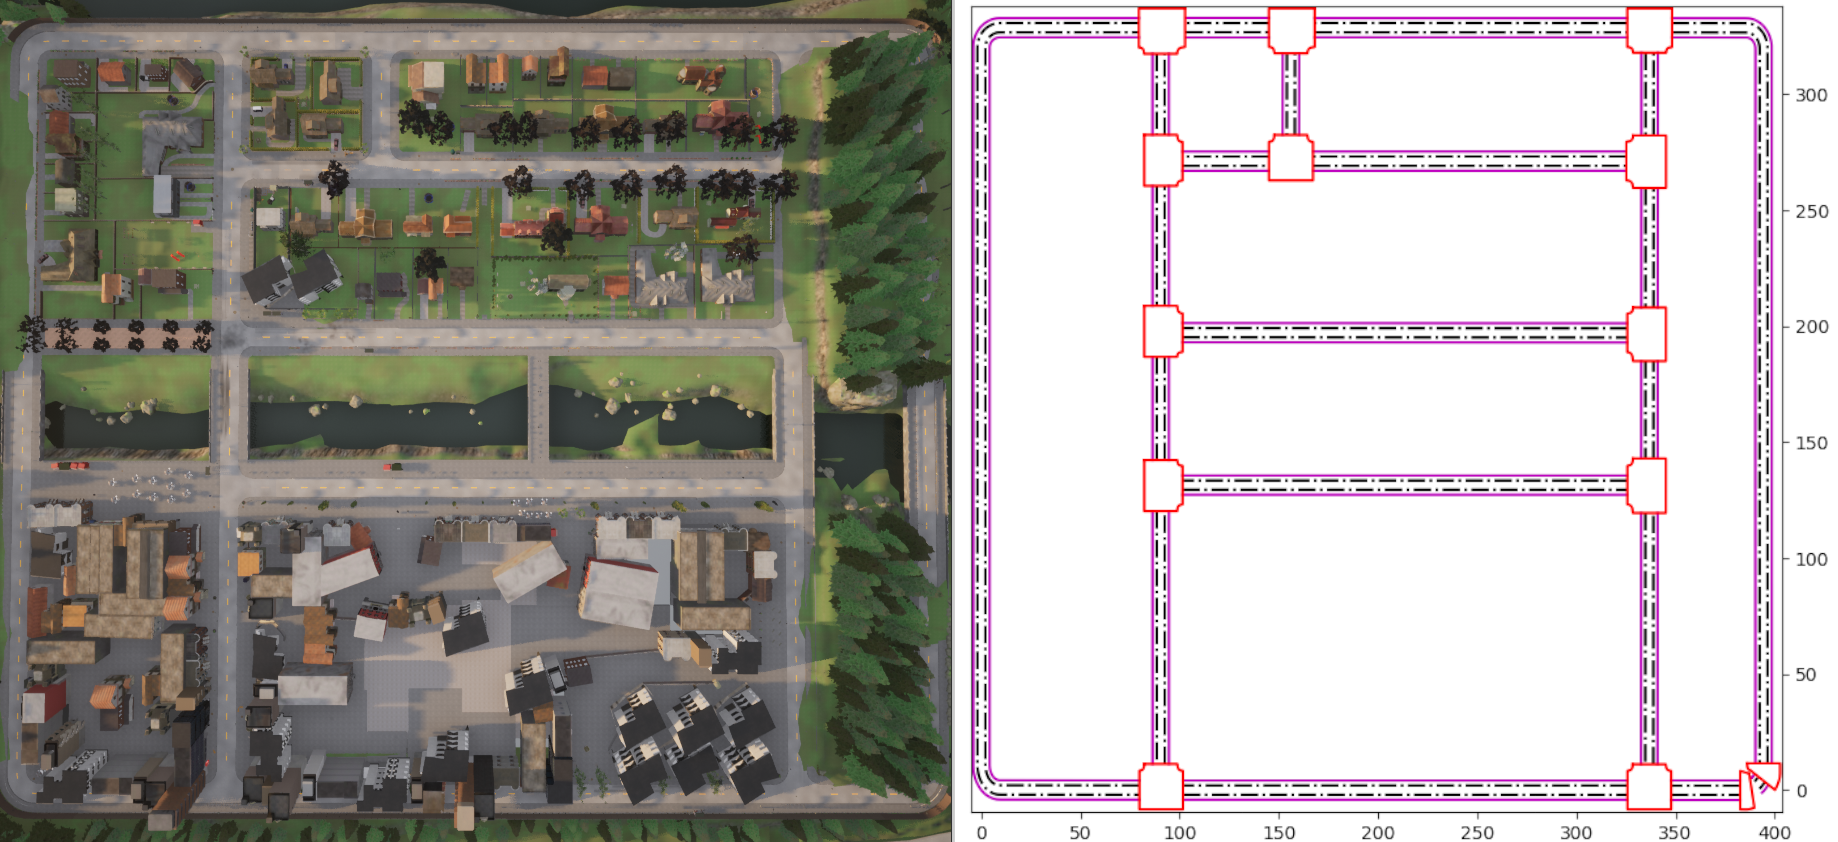
\includegraphics[width=1.0\textwidth]{chapter2/fig_town_map.png}
    \caption{The illustration of the road map in the simulator.}
    \label{fig:town_map}
\end{figure*}

The scheduling of model uploading in a vehicular federated learning system is considered, which consists of $M$ {\IAVs} deployed with multi-modal sensors.
Denote the set of {\IAVs} as $\carSet = \set{1, \dots, M}$.
Each {\IAV} collects the sensing data for the cooperative training of a deep neural network, e.g., SECOND \cite{SECOND}, in a federated learning manner \cite{FedAvg}.
This is one of the typical machine learning scenario in the application of autonomous driving as elaborated in \cite{icra2021-hong}.
In each training iteration, all the {\IAVs} first train their local models and then upload the trained models to an edge server for model aggregation via cellular uplink.
The aggregated model is then broadcast to the {\IAVs} for local training of next iteration until the convergence.
We particularly consider the uplink transmission scheduling in one iteration, where the {\IAVs}' mobility is exploited to save the transmission energy and suppress the model uploading time.

As an example illustrated in \figurename~\ref{fig:town_map}, $M$ {\IAVs} are distributed at different positions of a road network.
They are moving along predetermined routes respectively, but their velocities are time-varying and random.
The route of the $m$-th {\IAV} ($\forall m\in\carSet$) is quantized into a sequence of waypoints denoted as
\begin{align*}
    \tjSet_{m} \define \Paren{ \vec{w}_{m,1}, \dots, \vec{w}_{m,|\tjSet_{m}|} },
\end{align*}
where $\vec{w}_{m,i} \in \domR^2$ denotes the coordinates of the $i$-th waypoint,
$|\tjSet_m|$ denotes the cardinality of $\tjSet_m$.

The system time is organized by time slots, each with a duration of $T_s$ seconds.
In the $t$-th time slot, the location of the $m$-th {\IAV} is denoted as $\vec{d}_{m,t} \in \tjSet_{m}$, and the trajectory of the $m$-th {\IAV} is represented by its locations of the {\IAV} in all the time slots, denoted as
\begin{align*}
    \vec{L}_{m} \define \Paren{ \vec{d}_{m,1}, \vec{d}_{m,2}, \dots }.
\end{align*}
We approximate the trajectories of all {\IAVs} $\set{ \vec{L}_{m} | \forall m\in\carSet }$ as time-invariant Markov chains with the transition matrices
$\set{ \TransD_{m} \in \domR^{|\tjSet_{m}| \times |\tjSet_{m}|} | \forall m\in\carSet }$, where $\vec{D}_{m}$ represents the transition matrix of the $m$-th {\IAV}.
The entries of transition matrix $\TransD_{m}$ ($\forall m\in\carSet$) are defined as follows:
\footnote{
    A sufficient number of waypoints is selected for each route, such that the last waypoint is never reached at the end of the model uploading.
    For example, the uploading of the $m$-th {\IAV} always completes before arriving at the waypoint $\vec{w}_{m,|\tjSet_m|}$.
}
\begin{align}
     \Paren{\TransD_{m}}_{i,j} \define \Pr\Bracket{ \vec{w}_{m,j} | \vec{w}_{m,i} }, \forall i,j.
    \label{eqn:trans_mat}
\end{align}

Without loss of generality, the local model training and uploading of the considered iteration starts from the $1$-st time slot.
Due to the heterogeneous computation capabilities of the {\IAVs}, the local training time of the {\IAVs} may be different.
It is assumed that the local training time of the $m$-th {\IAV} is $T_{\text{comp},m}$, and the model consists of $U$ information bits.
Hence, an uplink queue with $U$ information bits is established at the $m$-th {\IAV} since the $(T_{\text{comp},m}+1)$-th time slot.
The period from the $1$-st time slot to the time slot that all the {\IAVs} complete their model uploading is referred to as the \emph{scheduling period} in the remaining of this chapter.
Thus, the length of the scheduling period depends on the uplink transmission scheduling.

All the {\IAVs} are served via a BS with $Y$ distributed antenna units,
and the locations of the antenna units are denoted as $\vec{b}_1, \dots, \vec{b}_Y$, respectively.
Each {\IAV} delivers its local model to the closest antenna unit, such that the transmission energy can be saved.
The distance between the $m$-th {\IAV} and the receiving antenna unit in the $t$-th time slot is denoted as
\begin{align*}
    l_{m,t} = \min_{i=1,2,\dots,Y} \|\vec{d}_{m,t} - \vec{b}_i\|_2.
\end{align*}
In order to avoid the co-channel interference, the {\IAVs} access the BS in a time-division manner in each time slot. There is at most one {\IAV} in the uplink transmission at any time instance. Let $\gamma_{m,t}$ be the ratio of the $t$-th time slot allocated to the $m$-th {\IAV}, we have
\begin{align*}
    \gamma_{m,t} \geq 0~\forall m\in\carSet \text{,~and} \sum_{m\in\carSet} \gamma_{m,t} \leq 1.
\end{align*}

Let $\mu_{m,t}$ be the path-loss of the $m$-th {\IAV}'s uplink channel in the $t$-th time slot, we have
\begin{align*}
    \mu_{m,t} = \kappa \bracket{ \frac{ \sigma }{ l_{m,t} } }^{\epsilon},
    % \label{eqn:mu}
\end{align*}
where $\kappa$ is a constant related to antenna characteristics, $\sigma$ is reference distance of the antenna far field, $\epsilon$ is the path-loss exponent.
Hence, the uplink throughput of the $m$-th {\IAV} in the $t$-th time slot $r_{m,t}$ is represented as follows:
\begin{align}
    r_{m,t} = \gamma_{m,t} T_s B_0
    \mathbb{E}_{h_{m,t}} \Bracket{
        \log_{2}\Paren{ 1 + \frac{|h_{m,t}|^2 \mu_{m,t} p_{m,t}}{N_0} }
    },
    \label{eqn:vu}
\end{align}
where $h_{m,t}$ is the coefficient of small-scale fading, $N_0$ is the power of Gaussian noise, $B_0$ is the uplink bandwidth, $p_{m,t}$ is the transmission power of the $m$-th {\IAV}, the expectation is taken over the random small-scale fading.
In the above equation, the ergodic capacity is used since the time slot is significantly longer than the channel coherent time.
Moreover, the transmission power should satisfy the following peak power constraint:
\begin{align*}
    p_{m,t} \leq P_{\max}.
\end{align*}

Let $u_{m,t}$ ($\forall, m,t$) be the remaining number of information bits in the uplink queue of the $m$-th {\IAV} in the $t$-th time slot, the queue dynamics are given by
\begin{align*}
    u_{m,t+1} = \max\Paren{ u_{m,t} - r_{m,t}, 0 }.
\end{align*}
Hence, the number of slots in the scheduling period, denoted by $T$, can be expressed as
\begin{align}
    T = \arg\min_{t} \indicator\Bracket{ \sum_{m\in\carSet} u_{m,t} \neq 0 }.
\end{align}


%=================================================================================================%
%=================================================================================================%

\section{Problem Formulation}
\label{sec:chapter2-formulation}
We would like to minimize the uplink energy consumption and model uploading time by exploiting the mobility of the {\IAVs}.
Because of their trade-off relation, the weighted summation of average uplink energy and uploading time (scheduling period duration) is used as the optimization objective.
Due to the randomness of {\IAVs}' trajectories, the joint scheduling design of the whole scheduling period, i.e., the transmission power and time allocation of all time slots, is a stochastic optimization problem, which can be formulated as a finite-horizon MDP.
We first define the system state, scheduling action, policy, and the cost function as follows.

\begin{definition}[State, Action and Policy]
    \label{def:mdp}
    In the $t$-th time slot, the local system state of the $m$-th {\IAV} is defined as
    \begin{align}
        \Stat_{m,t} &\define \Paren{ u_{m,t}, \vec{d}_{m,t} }, \forall m\in\carSet.
    \end{align}
    The global system state of the $t$-the time slot is defined as the aggregation of local system states of all {\IAVs}, thus
    \begin{align}
        \Stat_t &\define \Brace{ \Stat_{1,t}, \dots, \Stat_{M,t} }.
    \end{align}

    The scheduling action in the $t$-th time slot $\vec{A}_{t}$ consists of the allocation of transmission time and throughput%
    \footnote{
        Given the transmission time $\gamma_{m,t}$ and transmission power $p_{m,t}$,
        the throughput of the $m$-th {\IAV} in the $t$-th time slot $r_{m,t}$ can be determined according to Equation \eqref{eqn:vu}.
        We choose the transmission time and throughput as the action for the elaboration convenience.
    }
    of all {\IAVs},
    \begin{align}
        \vec{A}_{t} \define \Brace{ \gamma_{m,t}, r_{m,t} | \forall m\in\carSet }.
    \end{align}
    A centralized scheduling policy in the $t$-th time slot $\Policy_{t}$ is a mapping from the global system state $\Stat_{t}$ to the scheduling action, thus,
    \begin{align}
        \Policy_{t}\paren{\Stat_t} &= \Paren{ \Policy^{\Gamma}_{t}(\Stat_t), \Policy^{R}_{t}(\Stat_t) },
    \end{align}
    where $\Policy^{\Gamma}_{t}: \Stat_{t} \to \set{\gamma_{m,t} | m\in\carSet}$ denotes the throughput allocation policy and $\Policy^{R}_{t}: \Stat_{t} \to \set{r_{m,t} | m\in\carSet}$ denotes the time allocation policy.
\end{definition}

Given the action of the $t$-th time slot, the state transition probability from the $t$-th time slot to the $(t+1)$-th one is given by
\begin{align}
    &\Pr\Bracket{ \Stat_{t+1} | \Stat_{t}, \vec{A}_{t} } =
    % \nonumber\\
        \prod_{m\in\carSet} \Pr\Bracket{ \vec{d}_{m,t+1} | \vec{d}_{m,t} }
        \cdot \indicator\Bracket{ u_{m,t+1}=u_{m,t}+r_{m,t} },
    \label{eqn:trans_prob}
\end{align}
where $\Pr\bracket{ \vec{d}_{m,t+1} | \vec{d}_{m,t} }$ denotes the transition probability of the $m$-th {\IAV}'s trajectory from the waypoint $\vec{d}_{m,t}  \in \tjSet_{m}$ to $\vec{d}_{m,t+1} \in \tjSet_{m}$.

% It can be observed that different policies leads to different amount of uplink throughput, transmission energy consumption of each time slot, and finally different model uploading time and total energy consumption.
The policy design aims to minimize a weighted summation of the average model uploading time of all {\IAVs} and the average transmission energy consumption.
To achieve this goal, we define the system cost of the $t$-th time slot ($\forall t$) as follows:
\begin{align}
    g_{t}\Paren{ \Stat_{t}, \mathbf{A}_t } =
        \indicator\Bracket{ \sum\limits_{m\in\carSet} u_{m,t} > 0} +
        \omega \sum_{m\in\carSet} { \gamma_{m,t} p_{m,t} },
    \label{eqn:func_g}
\end{align}
where the two items on the right-hand-side (RHS) count the costs of uploading time and energy consumption, respectively, and $\omega$ is the weight on the energy consumption.

Hence, the expected overall cost of the whole scheduling period can be written as
\begin{align*}
    \widebar{G}\Paren{ \Policy_1,\dots,\Policy_\T } \define \mathbb{E}_{ \Stat_1,\dots,\Stat_\T } \Bracket{ \sum_{t=1}^{\T} g_{t}\paren{ \Stat_t, \vec{A}_t } },
\end{align*}
where $\T$ denotes the maximum tolerable number of time slots in one scheduling period.
As a result, the scheduling problem can be written as
\begin{align}
    \textbf{P1: } &\min_{\Policy_1, \dots, \Policy_\T} \widebar{G}\Paren{ {\Policy_1,\dots,\Policy_\T} }
    \label{eqn:p1_eqn}
    \\
    &\text{s.t.~~~~}
    \gamma_{m,t} \geq 0, \forall t, m\in\carSet
    \label{eqn:p1_cons_second}
    \\
    &~~~~~~\sum_{m\in\carSet} \gamma_{m,t} \leq 1, \forall t
    \label{eqn:p1_cons_last}
    \\
    &~~~~\sum_{ t=T_{\text{comp},m}+1 }^{\T} r_{m,t} \geq U, \forall m\in\carSet
    \\
    &~~~~p_{m,t} \leq P_{\max}, \forall t, m\in\carSet.
    \label{eqn:p1_cons_first}
\end{align}

In order to solve the above finite-horizon MDP, we first introduce the following Bellman's equations:
\begin{align}
    V_{t}(\Stat_t) =& \min_{\Policy_{t}(\Stat_t)} \Brace{ g_{t}\Paren{ \Stat_t, \vec{A}_t } +
    \sum_{\Stat_{t+1}} \Pr\Bracket{ \Stat_{t+1} | \Stat_{t}, \vec{A}_t } \cdot V_{t+1}(\Stat_{t+1})
    }, t=1,\dots,T,
    \label{eqn:p1_blm}
\end{align}
where
\begin{align}
    V_{t}(\Stat_{t}) \define \min_{\Policy_{t},\dots,\Policy_{\T}}& \mathbb{E}_{\Stat_{t},\dots,\Stat_{\T}}
    \Bracket{
        \sum_{\tau=t}^{\T} g_{\tau}\paren{ \Stat_{\tau}, \vec{A}_{\tau} } | \Stat_{t}
    }.
    \label{eqn:p1_val}
\end{align}
As a remark notice that in finite-horizon MDP, the optimal value functions can be heterogeneous for different time slots.

Hence, the optimal time and throughput allocation policies can be obtained by solving the RHS of equation \eqref{eqn:p1_blm}.
However, the problem {\bf P1} is difficult to solve.
On one hand, the transition probability of {\IAVs}' trajectories in Equation (\ref{eqn:trans_prob}) for a particular road network is hard to measure in advance, unless extensive real experiments can be conducted on the road network beforehand.
On the other hand, the optimal value functions depend on the global system state, which grows exponentially with respect to the number of {\IAVs}.

Thus, it is infeasible to calculate the value functions for each global system state before the online scheduling.
In order to address the above issues, a data-driven decentralized solution framework, namely {\fwName}, is proposed.
Particularly, the {\fwName} simulator is first proposed in Section \ref{sec:chapter2-framework} to obtain the waypoint transition probabilities.
Then the {\fwName} optimizer is proposed in Section \ref{sec:chapter2-new_framework} to address to issue of computation complexity in a decentralized manner.

\begin{figure*}[htp!]
    \centering
    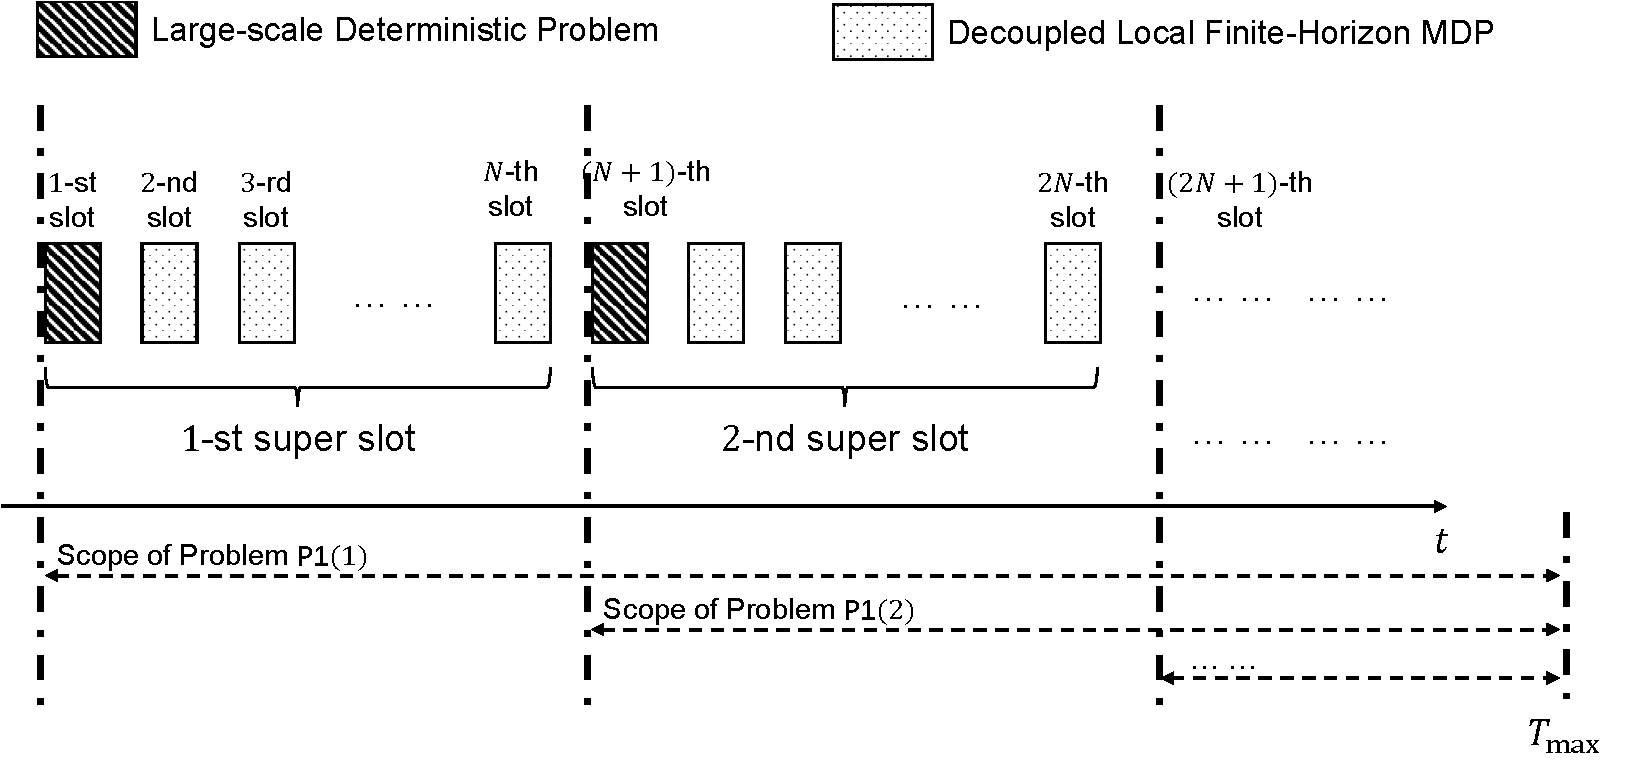
\includegraphics[width=1.0\textwidth]{chapter2/optimizer-framework.pdf}
    \caption{The illustration of the {\fwName} optimizer framework.}
    \label{fig:optimizer_framework}
\end{figure*}

\section{{\fwName} Simulator for Offline Transition Probability Training}
\label{sec:chapter2-framework}

The waypoint transition probabilities $\Pr\bracket{\vec{d}_{m,t+1}|\vec{d}_{m,t}}$ ($\forall m\in\carSet$) in \eqref{eqn:trans_prob} depend on the routes, the road topology, the microscopic traffic behaviors and etc, which are usually difficult to measure in advance.
A mismatching of the trajectories' statistics would lead to a biased estimation of the value function defined in \eqref{eqn:p1_val}, and degrade the performance of the optimized scheduling policy. To our best knowledge, there is currently no analytical model for the vehicles' trajectory prediction.
Therefore, we develop the {\fwName} simulator to simulate the trajectories of {\IAVs} for arbitrary traffic scenario, so that the waypoint transition probabilities $\Pr\bracket{\vec{d}_{m,t+1}|\vec{d}_{m,t}}$ can be trained in an offline manner.

The {\fwName} simulator integrates two well-known autonomous driving simulators, namely SUMO \cite{SUMO} and CARLA \cite{CARLA}.
CARLA is the open-source simulator based on Unreal Engine \cite{unrealengine}, which provides customized road topologies and vehicle types following the OpenDRIVE specification \cite{OpenDRIVE}.
On the other hand, SUMO provides the traffic management of vehicles with well-defined microscopic traffic flow model.
Based on them, the procedure to train the transition probabilities is given as follows.

\textbf{Road Topology and Traffic Initialization.} In order to simulate the random traffic on the particular scenario, we use CARLA to generate the target road map and leverage the program \emph{ActivityGen} provided by SUMO to generate random traffic demands according to the road map. The traffic demands can be customized by adjusting the following statistics: population distribution, working hours, car-holding rate, vehicular statistics and etc.
The study \cite{sumo-accuracy-mdpi} shows that the traffic flow generated by SUMO could match the traffic conditions of the real world on usual weekdays.

\textbf{Trajectory Dataset Generation.} Based on the above road map and traffic demands, the trajectories of all vehicles can be generated and recorded.
Let $\mathcal{X}_{m} $ be the set of vehicles running on the route of the $m$-th {\IAV} in all the simulation trials, and $$ \vec{x}^{(i)}_{m} = \Paren{ \vec{d}^{(i)}_{m,1}, \vec{d}^{(i)}_{m,2}, \dots }$$ be the trajectory of the $ i $-th vehicle in $\mathcal{X}_{m}$, where $\vec{d}^{(i)}_{m,t} \in \tjSet_{m}$ is the position in the $ t $-th time slot.

\textbf{Waypoint Transition Matrix Training.} Based on the trajectory dataset $ \{\vec{x}^{(i)}_{m}  | \forall i,m\} $, the waypoint transition matrices for all {\IAVs} $ \{\TransD_{m}| \forall m\} $ defined in \eqref{eqn:trans_mat} can be calculated as follows. 
\begin{align*}
    \Paren{\TransD_{m}}_{j,k} = 
        \frac{
            \sum_{t,i} \indicator\bracket{ \vec{d}^{(i)}_{t+1}=\vec{w}_{m,k}, \vec{d}^{(i)}_{t}=\vec{w}_{m,j} }
        }{
            \sum_{t,i}\sum_{l} \indicator \bracket{ \vec{d}^{(i)}_{t+1}=\vec{w}_{m,l}, \vec{d}^{(i)}_{t}=\vec{w}_{m,j} }
        }, \forall j,k.
\end{align*}
As a remark note that the trajectory dataset generation and waypoint transition matrix training are conducted in an offline manner before the uplink transmission, the {\fwName} simulator would have sufficient time to ensure a large number of trajectory samples. 

\begin{align}
    &\sum_{\tau=kN+1}^{T} g_{\tau}\Paren{
        \mathbb{E}_{\Stat_{\tau}} \Bracket{ \Stat_{\tau} | \Stat_{kN+1} }, \vec{A}_{\tau}
    }
    \nonumber\\
    \approx&~~T + \omega \sum_{\tau=kN+1}^{T} \sum_{m\in\carSet} \gamma_{m,\tau}
    2^\frac{r_{m,\tau}}{\gamma_{m,\tau}T_s B_0} 
    \times \xi_{m,\tau} \mathbb{E}_{\Stat_{\tau}} \Bracket{ l_{m,\tau}^{\epsilon}~|~\Stat_{kN+1} }
    \nonumber\\
    \define&~~F_k\Paren{ T, \mat{R}^{(k,T)}, \mat{\Gamma}^{(k,T)} }
    \label{eqn:fk}
\end{align}

\section{{\fwName} Optimizer: Online Decentralized Policy Optimization Framework}
\label{sec:chapter2-new_framework}

The joint policy optimization for the {\IAVs} in problem {\bf P1} suffers form the {\it curse of dimensionality}. This is because the transmission time and data rate allocation of each {\IAV} in each time slot depend on the global system state (aggregation of the states of all {\IAVs}), whose support grows exponentially with respect to the {\IAV} number.
It can be observed that if the transmission time allocation of all {\IAVs} $\{\gamma_{m,t}|\forall m,t\}$ is predetermined, the throughput allocation of each {\IAV} in all the time slots can be optimized without the consideration of other {\IAVs}' states.
However, fixing the transmission time allocation of all {\IAVs} before the model uploading would degrade the performance, as the transmission time allocation could not be adjusted according to the real-time positions and remaining information bits of all {\IAVs}.

In order to reduce the computation complexity and meanwhile maintain the performance gain of dynamic programming, a dynamic decoupling framework is proposed for the {\fwName} optimizer in this section. The framework is illustrated in \figurename~\ref{fig:optimizer_framework}, where every $N$ time slots is organized as a {\it super slot} and the online optimization consists of the following two time scales.
\begin{itemize}
    \item Super slot scale: the transmission time allocation of all {\IAVs} for the remaining time slots is periodically optimized at the beginning of each super slot. Such optimization will be approximated as a deterministic optimization problem based on the global system state at the beginning of each super slot.
    \item Slot scale: based on transmission time allocation, the optimization of throughput allocation policy of each {\IAV} for all the remaining time slots can be decoupled as a local finite-horizon MDP with tractable state space. The approximate expressions of local value functions will be derived, such that each {\IAV} can evaluate them and determine the throughput allocation in each slot without the effort of offline value iteration.
\end{itemize}

Without loss of generality, we consider the scheduling since the $k$-th super slot (from the $(kN+1)$-th time slot). The policy optimization of problem {\bf P1} for all the remaining time slots given the system state $\Stat_{kN+1}$ reduces to the following sub-problem:
\begin{align}
    \textbf{P1$(k)$:~~} &
    \min_{ \Policy_{kN+1}, \dots, \Policy_\T }
        \sum_{\tau=kN+1}^{\T}  \mathbb{E}_{\Stat_{\tau}} \Bracket{
            g_{\tau}\paren{ \Stat_{\tau}, \vec{A}_{\tau} } | \Stat_{kN+1}
        } \nonumber
    \\ \nonumber
    \text{s.t.~~} &\text{\eqref{eqn:p1_cons_second}, \eqref{eqn:p1_cons_last}, \eqref{eqn:p1_cons_first}},
    \\
    & \sum_{ \tau=\max\paren{kN+1,T_{\text{comp},m}} }^{ \T } r_{m,\tau} \geq {u}_{m,kN+1}, \forall m\in\carSet,
    \label{eqn:p1p_cons_last}
\end{align}
where the last constraint \eqref{eqn:p1p_cons_last} is to ensure all the data in the uplink queues of {\IAVs} should be delivered.


In the optimization of super slot scale, the average trajectories are used as the representatives to optimize the time slot allocation, such that the dynamic programming of problem \textbf{P1$(k)$} can be simplified to a deterministic optimization problem.
Note that
\begin{align}
    \sum_{\tau=kN+1}^{\T} g_{\tau}\Paren{
        \mathbb{E}_{\Stat_{\tau}}\Bracket{ \Stat_{\tau} | \Stat_{kN+1} }, \vec{A}_{\tau}
    }
    \label{eqn:cost_approx}
\end{align}
represents the system cost with the average trajectory
\begin{align}
    \Paren{
        \mathbb{E}\Bracket{ \vec{d}_{m,kN+1} | \vec{d}_{m,kN+1} },
        \dots,
        \mathbb{E}\Bracket{ \vec{d}_{m,T} | \vec{d}_{m,kN+1} }
    }
\end{align}
of the $m$-th {\IAV} ($\forall m\in\carSet$) since the $k$-th super slot. Approximating the objective by \eqref{eqn:cost_approx}, the policy optimization in problem \textbf{P1$(k)$} can be simplified into the following deterministic optimization of transmission time and throughput for the above average trajectories.
    \begin{align}
        \textbf{P2$(k)$:~} &
        ~~~\Paren{T^{(k,*)}, \mat{R}^{(k,*)}, \mat{\Gamma}^{(k,*)} }\nonumber \\
        & = \arg\min_{ T, \mat{R}^{(k,T)}, \mat{\Gamma}^{(k,T)} } F_k\Paren{ T, \mat{R}^{(k,T)}, \mat{\Gamma}^{(k,T)} }\nonumber
            \\
        &\text{s.t.~} \text{ \eqref{eqn:p1_cons_second}, \eqref{eqn:p1_cons_last}, \eqref{eqn:p1_cons_first},}
        \\
    & \sum_{ \tau=kN+1 }^{ T } r_{m,\tau} \geq {u}_{m,kN+1} \forall m\in\carSet, \label{eqn:constraint_T}
    \end{align}
where
$$
\mat{\Gamma}^{(k,T)} \define [ \gamma^{(k)}_{m,kN+\tau} ]_{1 \leq m \leq M, 1 \leq \tau \leq T-kN} \in \domR^{M \times (T-kN)}
$$
and
$$\mat{R}^{(k,T)} \define [ r^{(k)}_{m,kN+\tau}]_{1 \leq m \leq M, 1 \leq \tau \leq T-kN} \in \domR^{M \times (T-kN)}$$
are the aggregation matrices of time and throughput allocations of all the remaining time slots for the above average trajectories, respectively. $T$ denotes the number of slots in the scheduling period. $F_k(\cdot)$ is defined in Equation \eqref{eqn:fk}, where the high-SNR approximation on power consumption
\begin{align}
    p_{m,t} \approx \xi_{m,t} l_{m,t}^{\epsilon} 2^{\frac{ r_{m,t} }{ \gamma_{m,t} T_{s} B_0 }},
\end{align}
and $$\xi_{m,t} = \frac{N_0}{\kappa \sigma^\epsilon} 2^{-\mathbb{E}_{h_{m,t}}\bracket{\log_2{|h_{m,t}|^2}}}$$ is used.


The solution for the super slot scale optimization in problem \textbf{P2$(k)$} is discussed in Section \ref{sec:chapter2-kernel-policy}.
Its solution is denoted as
$$\mat{\Gamma}^{(k,*)}=[\gamma^{(k,*)}_{m,\tau+kN}]_{1 \leq m \leq M, 1 \leq \tau \leq T^{(k,*)}-kN}$$
and
$$\mat{R}^{(k,*)}=[r^{(k,*)}_{m,\tau+kN}]_{1 \leq m \leq M, 1 \leq \tau \leq T^{(k,*)}-kN}.$$
Moreover, $$\set{ \vecG{\gamma}^{(k,*)}_{m,\tau} | \forall m\in\carSet, \tau=kN+1,\dots,(k+1)N }$$ are adopted as the time allocation of the $k$-th super slot.

\noindent{\bf Remark:} {\it In high SNR region, with the reference time $\mat{\Gamma}^{(k,*)}$ and throughput allocations $\mat{R}^{(k,*)}$, the system cost with the average trajectory equals the average system cost with random trajectories. Thus,
\begin{align*}
F_k &\Paren{ T^{(k,*)}, \mat{R}^{(k,*)}, \mat{\Gamma}^{(k,*)}} =
\sum_{\tau=kN+1}^{T^{(k,*)}} \mathbb{E}_{\Stat_{\tau}} \Bracket{
            g_{\tau}\paren{ \Stat_{\tau}, \gamma^{(k,*)}_{m,\tau}, r^{(k,*)}_{m,\tau}} | \Stat_{kN+1}
        }.
\end{align*}
This will be exploited to derive a non-trivial performance bound of the proposed algorithm.}

In the optimization of slot scale, with the reference time allocation $\mat{\Gamma}^{(k,*)}$ and optimized length of scheduling period $T^{(k,*)}$, the throughput allocation policies of {\IAVs} can be decoupled. We first define the following local throughput allocation policies for the $m$-th {\IAV} ($\forall m\in\carSet$):
\begin{align}
    \Policy^{R}_{m,t}( \Stat_{m,t} ) = r_{m,t},~t=kN+1,\dots,T^{(k,*)}.
\end{align}
Moreover, the local reward function of the $m$-th {\IAV} is defined as
\begin{align}
    g_{m,t}\Paren{ \Stat_{m,t}, \Policy^{R}_{m,t}(\Stat_{m,t}) } = \gamma^{(k,*)}_{m,t} p_{m,t}.
\end{align}
Then the optimization of the local throughput allocation policies for the $m$-th {\IAV} can be written as follows:
\begin{align}
    \textbf{P3$(k,m)$:~}
    &\min_{ \set{\Policy^{R}_{m,\tau} | \tau=kN+1,\dots,T^{(k,*)} } }
        \nonumber\\
        &\sum_{\tau=kN+1}^{T^{(k,*)}}
        \mathbb{E}_{\Stat_{m,\tau}} \Bracket{
            g_{m,\tau}\Paren{ \Stat_{m,\tau}, \Policy^{R}_{m,\tau}( \Stat_{m,\tau} ) }\nonumber
        }
    \\\nonumber
    &\text{s.t.~} \text{ \eqref{eqn:p1_cons_second}, \eqref{eqn:p1_cons_last}, \eqref{eqn:p1_cons_first}, } \nonumber\\
    & ~~~ \sum_{ \tau=\max\paren{kN+1,T_{\text{comp},m}} }^{ T^{(k,*)}} r_{m,\tau} \geq {u}_{m,kN+1}.
\end{align}

Note that the above problem \textbf{P3$(k,m)$} is a finite-horizon MDP based on the local system state, it can be optimized locally at the $m$-th {\IAV}. The analytical expressions to approximate its local value functions will be proposed based on the reference time $\mat{\Gamma}^{(k,*)}$ and throughput allocation $\mat{R}^{(k,*)}$. Hence, at the beginning of each slot in the $k$-th super slot, the $m$-th {\IAV} first evaluates the next slot's local value function, and then determines the throughput allocation action of the current slot  according to the current local system state. The solution will be discussed in Section \ref{sec:chapter2-local-policy}.


%=================================================================================================%
%=================================================================================================%


\section{Global Super-Slot-Scale Optimization}
\label{sec:chapter2-kernel-policy}
The problem P2$(k)$ could be of a large scale when the number of remaining time slots is large. In this section, a large-scale optimization method is proposed.
Note that the time and throughput allocation ($\mat{\Gamma}^{(k,T)}, \mat{R}^{(k,T)}$) and scheduling period length $T$ are continuous and discrete, respectively, they can be optimized respectively. The optimization of P2$(k)$ given scheduling period length $T$ can be written as follows:
\begin{align}
    \textbf{P2$'(k,T)$:~}
    \min_{ \mat{R}^{(k,T)}, \mat{\Gamma}^{(k,T)} } &F_k\paren{ T, \mat{R}^{(k,T)}, \mat{\Gamma}^{(k,T)} }
    \\\nonumber
    \text{s.t.~} & \text{ \eqref{eqn:p1_cons_second}, \eqref{eqn:p1_cons_last}, \eqref{eqn:p1_cons_first}, \eqref{eqn:constraint_T} }.
\end{align}
Although the problem \textbf{P2$'(k,T)$} is convex, the conventional algorithms may not be applied due to huge complexity.
For example, the Newton interior method is of exponential computational complexity in the worst case \cite{monteiro1994}, which might be impractical for large $T$.
To address this issue, an acceleration gradient projection method \cite{Nesterov83} is adopted with convergence rate of $O(1/k^2)$ and computational complexity $O(k (M\T)^2)$, where $k$ denotes the number of iterations.

Let $\mat{R}^{(k,T)}_{0}, \mat{\Gamma}^{(k,T)}_{0}$ be an initial feasible solution satisfying the constraints \eqref{eqn:p1_cons_second}, \eqref{eqn:p1_cons_last}, \eqref{eqn:p1_cons_first}, and \eqref{eqn:constraint_T}.
Moreover, define
$$\mat{R}^{(k,T)}_{1}=\mat{R}^{(k,T)}_{0}, ~~\mat{\Gamma}^{(k,T)}_{1}=\mat{\Gamma}^{(k,T)}_{0}.$$
The problem \textbf{P2$'(k,T)$} can be solved by conducting the following two steps iteratively until convergence. 

\textbf{Step 1: Acceleration Point Calculation.}
In the $i$-th iteration ($i=1,2,3,\dots$), the acceleration points, denoted as $\widetilde{\mat{R}}^{(k,T)}_{i}$ and $\widetilde{\mat{\Gamma}}^{(k,T)}_{i}$, are chosen as the following linear combination of $(\mat{R}^{(k,T)}_{i}, \mat{R}^{(k,T)}_{i-1})$ and $(\mat{\Gamma}^{(k,T)}_{i}, \mat{\Gamma}^{(k,T)}_{i-1})$, respectively:
\begin{eqnarray*}
    &\widetilde{\mat{R}}^{(k,T)}_{i} &= \mat{R}^{(k,T)}_{i} + \frac{c_{i-1}-1}{c_{i}} \Paren{
        \mat{R}^{(k,T)}_{i} - \mat{R}^{(k,T)}_{i-1}
    }\nonumber
    \\
    &\widetilde{\mat{\Gamma}}^{(k,T)}_{i} &= \mat{\Gamma}^{(k,T)}_{i} + \frac{c_{i-1}-1}{c_{i}}  \Paren{
        \mat{\Gamma}^{(k,T)}_{i} - \mat{\Gamma}^{(k,T)}_{i-1} 
    },\nonumber
\end{eqnarray*}
where
\begin{align*}
    c_{0} = 1, c_{i} = \frac{1}{2} \Paren{ 1+\sqrt{ 1+4(c_{i-1})^2 } }.
\end{align*}

\textbf{Step 2: Update and Projection.}
Given the acceleration points, we define
$$\widebar{\mat{R}}^{(k,T)}_{i} = \widetilde{\mat{R}}^{(k,T)}_{i} - \eta \frac{\partial{F_k}}{\partial \mat{R}^{(k,T)}} \bigg|_{\widetilde{\mat{R}}^{(k,T)}_{i}}$$
and
$$\widebar{\mat{\Gamma}}^{(k,T)}_{i} = \widetilde{\mat{\Gamma}}^{(k,T)}_{i} - \eta \frac{\partial{F_k}}{\partial \mat{\Gamma}^{(k,T)}} \bigg|_{\widetilde{\mat{\Gamma}}^{(k,T)}_{i}}$$
where
\begin{align*}
    \frac{\partial{F_k}}{\partial \mat{R}^{(k,T)}} = \Bracket{
        &\xi_{m,\tau+kN} \mathbb{E}\bracket{ l_{m,\tau+kN}^{\epsilon} } \cdot
        2^{ \frac{r_{m,\tau+kN}}{\gamma_{m,\tau+kN} T_s B_0} }
        \nonumber\\
        &~~~~~~~~~~~~~~~~\cdot \paren{ \frac{\ln{2}}{T_s B_0} }
    }_{1 \leq m \leq M, 1 \leq \tau \leq T-kN},
    \\
    \frac{\partial{F_k}}{\partial \mat{\Gamma}^{(k,T)}} = \Bracket{
        &\xi_{m,\tau+kN} \mathbb{E}\bracket{ l_{m,\tau+kN}^{\epsilon} }
        \cdot 2^{ \frac{r_{m,\tau+kN}}{\gamma_{m,\tau+kN} T_s B_0} }
        \nonumber\\
        &\cdot \paren{1 - \frac{\ln{2}}{T_s B_0} \frac{r_{m,\tau+kN}}{\gamma_{m,\tau+kN}}}
    }_{1 \leq m \leq M, 1 \leq \tau \leq T-kN},
\end{align*}
 and $\eta$ is the constant gradient step size. Then the time and throughput allocations of the $i$-th iteration are updated as
\begin{align}
    \Paren{
        \mat{R}^{(k,T)}_{i+1}, &\mat{\Gamma}^{(k,T)}_{i+1}
    } = \mathcal{P}_{\C}\Paren{ \widebar{\mat{R}}^{(k,T)}_{i}, \widebar{\mat{\Gamma}}^{(k,T)}_{i} },
    \label{eqn:update_projection}
\end{align}
where $\mathcal{P}_{\C}$ denotes the projection of the matrix
$\widebar{\mat{R}}^{(k,T)}_{i}$ and $\widebar{\mat{\Gamma}}^{(k,T)}_{i}$
onto the constraint space $\C$ confined by equations \eqref{eqn:p1_cons_second}, \eqref{eqn:p1_cons_last}, \eqref{eqn:p1_cons_first} and \eqref{eqn:constraint_T}.

Specifically, let $\widebar{\gamma}^{(k,i)}_{m,\tau}$ and $\widebar{r}^{(k,i)}_{m,\tau}$ be the $(m,\tau)$-th entries of the matrices $\widebar{\mat{\Gamma}}^{(k,T)}_{i}$ and $\widebar{\mat{R}}^{(k,T)}_{i}$, respectively, the projection in Equation \eqref{eqn:update_projection} is equivalent to the following minimization problem:
\begin{align}
    \Paren{ \mat{R}^{(k,T)}_{i+1}, \mat{\Gamma}^{(k,T)}_{i+1} }
    = &\arg\min_{ \paren{ \mat{R},\mat{\Gamma} } \in \C }
            \nonumber\\
            &
            \sum_{m\in\carSet} \sum_{\tau=kN+1}^{T}
            \paren{ \widebar{\gamma}^{(k,i)}_{m,\tau} - \gamma_{m,\tau} }^{2} +
            \paren{ \widebar{r}^{(k,i)}_{m,\tau} - r_{m,\tau} }^{2}.
    \label{eqn:simplex_projection}
\end{align}
According to the proposition 2 of \cite{fast-projection}, the solution to the above projection problem is summarized in the following lemma.
\begin{lemma}[Alternative Projection Onto Simplex and Hyperplane]
    Let $\set{ \bar{\gamma}^{(m)}_{\tau} | \forall m\in\carSet }$ denote the descent sorting of $\set{ \bar{\gamma}^{(k,i)}_{m,\tau} | \forall m\in\carSet }$ in the $\tau$-th time slot ($\tau=kN+1,\dots,T$)
    ,
    and
    $\set{ \bar{r}^{(\tau)}_{m} | \tau=1,2,\dots,T-kN }$ denote the descent sorting of $\set{\bar{r}^{(k,i)}_{m,\tau} | \tau=kN+1,\dots,T}$ for the $m$-th {\IAV}.
    Thus,
    $\bar{\gamma}^{(1)}_{\tau} \geq \dots \geq \bar{\gamma}^{(M)}_{\tau}$ and $\bar{r}^{(1)}_{m} \geq \dots \geq \bar{r}^{(T-kN)}_{m}$.
    The solution of Equation \eqref{eqn:simplex_projection} is given by
    $\mat{\Gamma}^{(k,T)}_{i+1} = [\gamma^{(k,i+1)}_{m,kN+\tau}]_{1 \leq m \leq M, 1 \leq \tau \leq T-kN}$ and $\mat{R}^{(k,T)}_{i+1} = [r^{(k,i+1)}_{m,kN+\tau}]_{1 \leq m \leq M, 1 \leq \tau \leq T-kN}$.
    Moreover,
    \begin{align}
        \gamma^{(k,i+1)}_{m,\tau} = \Bracket{ \widebar{\gamma}^{(k,i)}_{m,\tau} &- \frac{\sum_{j=1}^{m'}\bar{\gamma}^{(j)}_{\tau} - 1}{m'} }^{+}
        \\
        r^{(k,i+1)}_{m,\tau} = \min\Paren{
            \Bracket{ \widebar{r}^{(k,i)}_{m,\tau} &- \frac{\sum_{j=1}^{\tau'}u_{m,t} - \bar{r}^{(j)}_{m}}{\tau'} }^{+},
            \nonumber\\
            &T_s B_0 \log_2\paren{ \frac{P_{\max}}{ \xi_{m,\tau} \mathbb{E}[l^{\epsilon}_{m,\tau}]}} \gamma^{(k,i+1)}_{m,\tau}
        }
    \end{align}
    where
    $$m' = \max_{m} \set{m: {\sum_{j=1}^{m} \bar{\gamma}^{(j)}_{\tau} - 1 } <{m} \bar{\gamma}^{(m)}_{\tau}},$$ 
    $$\tau' = \max_{\tau} \set{\tau: {\sum_{j=1}^{\tau} u_{m,t} - \bar{r}^{(j)}_{m}} <{\tau} \bar{r}^{(\tau)}_{m}}.$$
\end{lemma}

Denote ${\mat{\Gamma}^{(k,T,*)}}$ and ${\mat{R}^{(k,T,*)}}$ as the optimized time and throughput allocations of problem \textbf{P2$'(k,T)$} after convergence, the optimization of scheduling period duration can be written as follows.
\begin{align}
    \textbf{P2$''(k)$:~} & \min_{T} F_{k}  \Paren{T, {\mat{\Gamma}^{(k,T,*)}}, {\mat{R}^{(k,T,*)}} }.
    \label{eqn:p2pp_k}
\end{align}
Note that the variable $T$ is an integer between $1$ and $\T$, a  bisection search algorithm is elaborated below to solve problem \textbf{P2$''(k)$}. Finally, the optimized scheduling period duration $T$ in problem \textbf{P2$''(k)$} is denoted as $T^{(k,*)}$, the corresponding optimized time and throughput allocations are denoted as $\mat{\Gamma}^{(k,*)}$ and  ${\mat{R}^{(k,*)}}$ respectively. 
\begin{algorithm}[ht]
    \caption{Bisection Search Algorithm for problem \textbf{P2$''(k)$}}\label{alg_bnb}
    \DontPrintSemicolon
    \KwOut{ $T^{(k,*)}$ }
    % \KwOut{$\{ { \gamma^{*}_{m,\tau} }, { r^{*}_{m,\tau} } | \forall m\in\carSet, \tau=kN+1,\dots,{T}^{*} \}$}
    $\tau_{l} \gets kN+1$, $\tau_{r} \gets \T$\;
     $w_{r} \gets \min F_{k}( \tau_{r}, \mat{R}_{r}, \mat{\Gamma}_{r} )$ by solving \textbf{P2$'( k,\tau_{r} )$}\;
    \While{ $\tau_{r} - \tau_{l} > 1$ }
    {
        $\tau_{mid} \gets \lfloor{ (\tau_{l} + \tau_{r})/2 }\rfloor$\;
        $w_{mid} \gets \min F_{k}( \tau_{mid}, \mat{R}_{mid}, \mat{\Gamma}_{mid} )$ by solving \textbf{P2$'( k,\tau_{mid} )$}\;
        \If{ $w_{r} - w_{mid} < 0$ }{
            $\tau_{l} \gets \tau_{mid}$\; %g(x)/energy domains, moves right
        }
        \Else{
            $\tau_{r} \gets \tau_{mid}$\; %f(x)/time domains, moves left
            $w_{r} \gets w_{mid}$\;
        }
    }
    \Return{ $T^{(k,*)} \gets \tau_{l}$ }\;
\end{algorithm}

\section{Local Slot-Scale Optimization}
\label{sec:chapter2-local-policy}

In this section, the low-complexity algorithm solving the problem \textbf{P3$(k,m)$} without the offline value iteration is elaborated. Note that the local system state of the $m$-th {\IAV} consists of $\Stat_{m,t} =  ( u_{m,t}, \vec{d}_{m,t} )$, the Bellman's equations of problem \textbf{P3$(k,m)$} are given below.
\begin{align*}
    V_{m,t} & \paren{  u_{m,t}, \vec{d}_{m,t} }=
    \min_{ r_{m,t} } \gamma^{(k,*)}_{m,t} p_{m,t} + \mathbb{E}_{ \vec{d}_{m,t+1} } V_{m,t+1}\paren{  u_{m,t}-r_{m,t}, \vec{d}_{m,t+1} },
\end{align*}
where the transmission power $p_{m,t}$ is a function of $\gamma^{(k,*)}_{m,t}$, $\vec{d}_{m,t}$ and $r_{m,t}$, and the local value function of the $m$-th {\IAV} in the $t$-th time slot is given by
\begin{align}
    V_{m,t} & (u_{m,t}, \vec{d}_{m,t}) \define 
    \min_{ \{\Policy^{R}_{m,t}|\forall t\} } \mathbb{E} \Bracket{ \sum_{\tau=t}^{T^{(k,*)}} g_{m,t}(u_{m,t}, \vec{d}_{m,t}, \Policy^{R}_{m,t}) }.
\end{align}
For the notation convenience, we define
\begin{align}
    \widetilde{V}_{m,t+1}\paren{u_{m,t+1}, \vec{d}_{m,t}} = \mathbb{E}_{ \vec{d}_{m,t+1} | \vec{d}_{m,t} } V_{m,t+1}\paren{  u_{m,t+1}, \vec{d}_{m,t+1} }.
 \label{eqn:local_valfn_alt}
\end{align}
Hence, given the local value function and local system state, the optimal throughput allocation of the $m$-th {\IAV} in the $t_i$-th time slot, where  $t_i = kN + i$ and $i=1,2,\dots,N$, can be obtained via the following optimization problem.
\begin{align}
    \min_{ r_{m,t_i} } \gamma^{(k,*)}_{m,t_i} p_{m,t_i} (r_{m,t_i})+ \widetilde{V}_{m,t_i+1}\paren{u_{m,t_i}-r_{m,t_i}, \vec{d}_{m,t_i}}.
    \label{eqn:local_valfn}
\end{align}

Although the dimension of local value function is much less than the global optimization in Equation \eqref{eqn:p1_blm},
the complexity of evaluating local value functions $V_{m,t}  (u_{m,t}, \vec{d}_{m,t})$ ($\forall t, u_{m,t}, \vec{d}_{m,t}$) or equivalently $\widetilde{V}_{m,t}(\cdot)$ is still high. Therefore, we propose a novel method to approximate the local value functions with the analytical expressions based on the reference throughput allocation. 
Let
$$\paren{ r^{(k,i-1)}_{m,t_i}, r^{(k,i-1)}_{m,t_i+1}, \dots, r^{(k,i-1)}_{m,T^{(k,*)}} }$$
with 
\begin{align}
    \sum_{\tau=t_i}^{T^{(k,*)}} r^{(k,i-1)}_{m,\tau} = u_{m,t_i}
    \label{eqn:reference_constraint}
\end{align}
be the reference throughput allocation for all the remaining time slots in the optimization of the $t_i$-th time slot, and
\begin{align*}
    \slide{r}^{(k,i-1)}_{m} = \paren{ r^{(k,i-1)}_{m,t_i+1}, r^{(k,i-1)}_{m,t_i+2}, \dots, r^{(k,i-1)}_{m,T^{(k,*)}} }
\end{align*}
be the corresponding reference throughput allocation for the future time slots. The optimization in Equation \eqref{eqn:local_valfn} can be equivalently written as
\begin{align}
\textbf{P3$'(k,m,t_i)$:}& \min_{ \Delta r_{m,t_i} } \gamma^{(k,*)}_{m,t_i} p_{m,t_i} (r^{(k,i-1)}_{m,t_i}+\Delta r_{m,t_i}) \nonumber\\ 
 +~&\widetilde{V}_{m,t_i+1}\paren{u_{m,t_i}-r^{(k,i-1)}_{m,t_i}-\Delta r_{m,t_i}, \vec{d}_{m,t_i}}.  \label{eqn:local_valfn_delta}
 \\
 \text{s.t.~}& p_{m,t_i}( r^{(k,i-1)}_{m,t_i} + \Delta{r}_{m,t_i} ) \leq P_{\max}
\end{align}

\subsection{Local Value Function Approximation}
\label{subsec:chapter2-local_valfn_approx}

In this section, we approximate the expected local value function $\widetilde{V}_{m,t_i+1}\paren{\cdot}$ in Equation \eqref{eqn:local_valfn_delta} via the reference throughput allocations $\slide{r}^{(k,i-1)}_{m}$.
Let 
\begin{align}
    \widebar{G}_{m,t_i+1} & \paren{ \slide{r}^{(k,i-1)}_{m}, \vec{d}_{m,t_i} }
    \define
    \sum_{\tau=t_i+1}^{T^{(k,*)}}
    \mathbb{E}_{\vec{d}_{m,\tau}}\Bracket{
        \gamma^{(k,*)}_{m,\tau} p_{m,\tau}\paren{ r_{m,\tau}^{(k,i-1)}}
        ~|~\vec{d}_{m,t_i}
    }
\end{align}
denote the expected cost of $m$-th {\IAV} since the $(t_i+1)$-th time slot with the reference throughput allocations $\slide{r}^{(k,i)}_{m} $ given the current location $\vec{d}_{m,t_i}$, and
$$
\Delta{\slide{r}^{(k,i)}_{m}} = (\Delta{r}_{m,t_i+1},\dots,\Delta{r}_{m,T^{(k,*)}})
$$
be the adjustment on the reference throughput allocation.
We approximate the expected local value function $\widetilde{V}_{m,t_i+1}\paren{\cdot}$ in Equation \eqref{eqn:local_valfn_delta} as follows:
\begin{align}
    \widetilde{V}_{m,t_i+1} & ( u_{m,t_i} -r^{(k,i-1)}_{m,t_i} -\Delta{r}_{m,t_i}, \vec{d}_{m,t_i} )  \approx
    \nonumber\\
     \min_{\Delta{\slide{r}^{(k,i)}_{m}}} & ~~~\widebar{G}_{m,t_i+1}\Paren{ \slide{r}^{(k,i-1)}_{m} + \Delta{\slide{r}^{(k,i)}_{m}}, \vec{d}_{m,t_i} }
    \nonumber\\
    \text{s.t.~} & ~~~ \sum_{\tau=t_i+1}^{T^{(k,*)}} \Delta{r}_{m,\tau} = \Delta{r}_{m,t_i}
    \nonumber\\
    & ~~~ \Delta{r}_{m,t_i} \times \Delta{r}_{m,\tau} \geq 0, \forall \tau = {t_i+1},\dots, T^{(k,*)}. \nonumber
\end{align}
The above first constraint is to ensure that the total number of transmission bits is $u_{m,t_i}$, and the second constraint is to limit the search space of $\Delta{\slide{r}^{(k,i)}_{m}}$. Moreover, we have the following conclusion on its asymptotic optimal solution.

\begin{lemma}
    \label{lemma:local_rate_opt}
    Define the following indexes of time slots:
     \begin{align}
        \hat{\tau}_{m} &= \arg\max_{\tau} \mathbb{E}\Bracket{ l_{m,\tau}^{\epsilon}~|~\vec{d}_{m,t_i} }
                          \cdot 2^{\frac{r^{(k,i)}_{m,\tau}}{T_s B_0 \gamma^{(k,*)}_{m,\tau}}},
        \\
        \breve{\tau}_{m} &= \arg\min_{\tau} \mathbb{E}\Bracket{ l_{m,\tau}^{\epsilon}~|~\vec{d}_{m,t_i} }
                          \cdot 2^{\frac{r^{(k,i)}_{m,\tau}}{T_s B_0 \gamma^{(k,*)}_{m,\tau}}}.
    \end{align}   
    For sufficiently small $\Delta{r}_{m,t_i}$, the following solution is asymptotically optimal:
    \begin{itemize}
        \item If $\Delta{r}_{m,t_i} > 0$, all the entries of $\Delta{\slide{r}^{(k,i)}_{m}}$ is $0$ except that $\Delta{r}_{m,\hat{\tau}_{m}} = \Delta{r}_{m,t_i}$;
        \item If $\Delta{r}_{m,t_i} < 0$, all the entries of $\Delta{\slide{r}^{(k,i)}_{m}}$ is $0$ except that $\Delta{r}_{m,\breve{\tau}_{m}} = \Delta{r}_{m,t_i}$;
    \end{itemize}
\end{lemma}
\begin{proof}
    The original optimization problem is convex, and we discuss the solution depending on the sign of $\Delta{r}_{m,t_i}$ in the following two cases.

    In the case when $\Delta{r}_{m,t_i} \leq 0$, we have $\Delta{r}_{m,\tau} \geq 0$ ($\tau=t_i+1, \dots, T^{(k,*)}$).
    Therefore, let $\lambda \in \domR_+$ and $\vecG{\mu} \in \domR^{(T^{(k,*)}-t_i)}_+$ denote the Lagrangian multipliers, the corresponding Lagrangian function of the convex optimization problem is given as follows:
    \begin{align*}
        L( \Delta{\slide{r}}^{(k,i)}_{m}, \lambda, \vecG{\mu} ) =
        &\sum_{\tau=t_i+1}^{T^{(k,*)}} \gamma^{(k,*)}_{m,\tau} p_{m,\tau}( r^{(k,i)}_{m,\tau} - \Delta{r}_{m,\tau} )
        \nonumber\\
        &+ \lambda \Paren{ \sum_{\tau=t_i+1}^{T^{(k,*)}} \Delta{r}_{m,\tau} - \Delta{r}_{m,t_i} }
        - \sum_{j=1}^{T^{(k,*)}-t_i} \mu_{j} \Delta{r}_{m,t_i+j}.
    \end{align*}

    The Karush-Kuhn-Tucker (KKT) conditions for the original convex optimization problem are:
    \begin{enumerate}
        \item primal constraints: $\sum_{\tau=t_i+1}^{T^{(k,*)}} \Delta{r}_{m,\tau} - \Delta{r}_{m,t_i} \leq 0$, $\Delta{\slide{r}}^{(k,i)}_{m} \vecG{\mu}^T = 0$;
        \item dual constraints: $\lambda \geq 0$;
        \item complementary slackness:
        $$
        \lambda (\sum_{\tau=t_i+1}^{T^{(k,*)}} \Delta{r}_{m,\tau} - \Delta{r}_{m,t_i}) = 0;
        $$
        \item stationarity:
        $$
        \nabla_{\Delta{\slide{r}}^{(k,i)}_{m}} L( \Delta{\slide{r}}^{(k,i)}_{m}, \lambda, \vec{\mu} )
        = \vec{0},
        $$
        i.e.,
        $$
        - \frac{\ln{2}}{T_s B_0} \mathbb{E}[l^{\epsilon}_{m,t_i+j}] \cdot 2^{\frac{r^{(k,i)}_{m,t_i+j} - \Delta{r}_{m,t_i+j}}{T_s B_0 \gamma^{(k,*)}_{m,t_i+j}}} + \lambda - \mu_j = 0,
        \forall j.
        $$
    \end{enumerate}

    Notice that $\Delta{\slide{r}}^{(k,i)}_{m} \vecG{\mu}^T = 0$ is always true for optimal solution, we have the following statements:
    \begin{itemize}
        \item if $\mu_j > 0$, then $\Delta{r}_{m,t_i+j} = 0$, which implies
        $$
        \lambda < \frac{\ln{2}}{T_s B_0} \mathbb{E}[l^{\epsilon}_{m,t_i+j}] \cdot 2^{\frac{r^{(k,i)}_{m,t_i+j}}{T_s B_0 \gamma^{(k,*)}_{m,t_i+j}}}.
        $$
        For the corresponding contrapositive statement, we have: if $\lambda \geq \frac{\ln{2}}{T_s B_0} \mathbb{E}[l^{\epsilon}_{m,t_i+j}] \cdot 2^{\frac{r^{(k,i)}_{m,t_i+j}}{T_s B_0 \gamma^{(k,*)}_{m,t_i+j}}}$, then $\Delta{r}_{m,t_i+j} > 0$.
        \item if $\mu_j = 0$, then $\Delta{r}_{m,t_i+j} \geq 0$, and we have
        $$
        \Delta{r}_{m,\tau} = - r^{(k,i)}_{m,\tau} + T_s B_0 \gamma^{(k,*)}_{m,\tau} \log_2{\frac{T_s B_0 \lambda}{\ln{2} \mathbb{E}[l^{\epsilon}_{m,\tau}]}}.
        $$
    \end{itemize}

    Therefore, for sufficiently small $\Delta{r}_{m,t_i}$, the index of non-zero rate allocation is the {\it largest} one satisfying the constraint w.r.t $\lambda$, i.e.,
    $$
    \hat{\tau}_{m} = \arg\max_{\tau} \mathbb{E}\Bracket{ l_{m,\tau}^{\epsilon}~|~\vec{d}_{m,t_i} }
                            \cdot 2^{\frac{r^{(k,i)}_{m,\tau}}{T_s B_0 \gamma^{(k,*)}_{m,\tau}}}.
    $$

    Similarly, in the case when $\Delta{r}_{m,t_i} \ge 0$, let $\Delta{\slide{r}}^{(k,i)'}_{m} = - \Delta{\slide{r}}_{m,t_i}$, we have the Lagrangian function $L'(\cdot)$ w.r.t $\Delta{\slide{r}}^{(k,i)'}_{m,t_i}$ as follows:
    \begin{align*}
        &L'( \Delta{\slide{r}}^{(k,i)'}_{m}, \lambda, \vecG{\mu} ) =
        \sum_{\tau=t_i+1}^{T^{(k,*)}} \gamma^{(k,*)}_{m,\tau} p_{m,\tau}( r^{(k,i)}_{m,\tau} + \Delta{r}'_{m,\tau} )
        \nonumber\\
        &- \lambda \Paren{ \sum_{\tau=t_i+1}^{T^{(k,*)}} \Delta{r}_{m,\tau} - \Delta{r}_{m,t_i} }
        - \sum_{j=1}^{T^{(k,*)}-t_i} \mu_{j} \Delta{r}_{m,t_i+j}.
    \end{align*}
    Therefore, the only difference compared to the analysis in previous case exists in stationarity constraint, where
    $$
    \frac{\ln{2}}{T_s B_0} \mathbb{E}[l^{\epsilon}_{m,t_i+j}] \cdot 2^{\frac{r^{(k,i)}_{m,t_i+j} - \Delta{r}'_{m,t_i+j}}{T_s B_0 \gamma^{(k,*)}_{m,t_i+j}}} + \lambda - \mu_j = 0,
        \forall j.
    $$
    For sufficiently small $\Delta{r}_{m,t_i}$, the index of non-zeros rate allocation is the {\it smallest} one, i.e.,
    $$
    \breve{\tau}_{m} = \arg\min_{\tau} \mathbb{E}\Bracket{ l_{m,\tau}^{\epsilon}~|~\vec{d}_{m,t_i} }
                            \cdot 2^{\frac{r^{(k,i)}_{m,\tau}}{T_s B_0 \gamma^{(k,*)}_{m,\tau}}}.
    $$
\end{proof}
As a result, the expected approximate value function can be approximated as follows.
\begin{align}
    &\widetilde{V}_{m,t_i+1}\paren{ u_{m,t_i}-r^{(k,i-1)}_{m,t_i}-\Delta{r}_{m,t_i}, \vec{d}_{m,t_i} }
    \nonumber\\
    &\approx
    \begin{cases}
        \widebar{G}_{m,t_i+1}\paren{ \slide{r}^{(k,i-1)}_{m} + \vec{e}_{\hat{\tau}_{m}} \Delta{r}_{m,t_i}, \vec{d}_{m,t_i} }, & \Delta{r}_{m,t_i} > 0
        \\
        \widebar{G}_{m,t_i+1}\paren{ \slide{r}^{(k,i-1)}_{m} + \vec{e}_{\breve{\tau}_{m}} \Delta{r}_{m,t_i}, \vec{d}_{m,t_i} }, & \Delta{r}_{m,t_i} < 0
    \end{cases}. \label{eqn:local-value-app}
\end{align}
In the above expressions, $\vec{e}_{\tau}$ denotes the vector whose $\tau$-th dimension is one and other dimensions are zero.

\subsection{Online Scheduling}
\label{subsec:chapter2-local_opt}
With the local value function approximation in the previous section, the local throughput allocation of the $m$-th {\IAV} in the $t_i$-th slot can be determined by solving problem \textbf{P3$'(k,m,t_i)$}. We first introduce the following conclusion.
\begin{lemma}
    \label{lemma:local_approx_solution}
    With the approximation of local value function in Equation \eqref{eqn:local-value-app}, the optimal solution of problem \textbf{P3$'(k,m,t_i)$} is within the set $\{f_{m,t_i}(\hat{\tau}_m),f_{m,t_i}(\breve{\tau}_m) \}$, where
    \begin{align}
        f_{m,t_i}(\tau_m) \define
        \min\Paren{
            &\frac{
                T_s B_0 \gamma^{(k,*)}_{m,t_i} \gamma^{(k,*)}_{m,\tau} \paren{ \log_2{ \mathbb{E}[l^{\epsilon}_{m,\tau_m}] } - \log_2{l^{\epsilon}_{m,t_i}} } 
            }{
                \gamma^{(k,*)}_{m,t_i} + \gamma^{(k,*)}_{m,\tau_m}
            }
            \nonumber\\
            &+\frac{
                r^{(k,*)}_{m,\tau_m}\gamma^{(k,*)}_{m,t_i} - r^{(k,*)}_{m,t_i}\gamma^{(k,*)}_{m,\tau_m} 
            }{
                \gamma^{(k,*)}_{m,t_i} + \gamma^{(k,*)}_{m,\tau_m}
            },
            \Delta{r}^{\max}_{m,t_i}
        },
    \end{align}
    where $p_{m,t_i}( r^{(k,i-1)}_{m,t_i} + \Delta{r}^{\max}_{m,t_i} ) = P_{\max}$.
\end{lemma}
\begin{proof}
    Note that given the fixed solution $\tau$, the corresponding optimal rate allocation is given as follows:
    \begin{align*}
        \min_{ \Delta{r}_{m,t_i} } &\gamma^{(k,*)}_{m,t_i} p_{m,t_i}( r^{(k,i)}_{m,t_i} + \Delta{r}_{m,t_i} )
            + \gamma^{(k,*)}_{m,\tau} p_{m,\tau}( r^{(k,i)}_{m,\tau} - \Delta{r}_{m,t_i} )
    \end{align*}
    The solution to the above optimization problem is easy to obtain by taking the derivative w.r.t $\Delta{r}_{m,t_i}$ and setting it to zero, i.e.,
    $$
    \frac{\ln{2}}{T_s B_0} l^{\epsilon}_{m,t_i} 2^{\frac{r^{(k,i)}_{m,t_i} + \Delta{r}_{m,t_i}}{T_s B_0 \gamma^{(k,*)}_{m,t_i}}}
    + \frac{\ln{2}}{T_s B_0} \mathbb{E}[l^{\epsilon}_{m,\tau}] 2^{\frac{r^{(k,i)}_{m,\tau} - \Delta{r}_{m,t_i}}{T_s B_0 \gamma^{(k,*)}_{m,\tau}}} = 0,
    $$
    and the solution is
    \begin{align*}
        \Delta{r}_{m,t_i} =
        &\frac{
            T_s B_0 \gamma^{(k,*)}_{m,t_i} \gamma^{(k,*)}_{m,\tau} \paren{ \log_2{ \mathbb{E}[l^{\epsilon}_{m,\tau}] } - \log_2{l^{\epsilon}_{m,t_i}} } 
        }{
            \gamma^{(k,*)}_{m,t_i} + \gamma^{(k,*)}_{m,\tau}
        }
        \nonumber\\
        &+ \frac{
            r^{(k,*)}_{m,\tau}\gamma^{(k,*)}_{m,t_i} - r^{(k,*)}_{m,t_i}\gamma^{(k,*)}_{m,\tau} 
        }{
            \gamma^{(k,*)}_{m,t_i} + \gamma^{(k,*)}_{m,\tau}
        }.
    \end{align*}
\end{proof}

Hence, the optimized throughput allocation of the $m$-th {\IAV} in the $t_i$-th slot is denoted by
\begin{align}
    r^{(k,i)}_{m,t_i} = r^{(k,i-1)}_{m,t_i}+f_{m,t_i}(\tau_m^*), \label{eqn:throughput}
\end{align}
where 
\begin{align}
    \tau_m^*=\arg \min_{ \tau_m\in \{\hat{\tau}_m,\breve{\tau}_m\} } &\gamma^{(k,*)}_{m,t_i} p_{m,t_i} (r^{(k,i-1)}_{m,t_i}+f_{m,t_i}(\tau_m)) \nonumber\\
 & + \widebar{G}_{m,t_i+1}\paren{ \slide{r}^{(k,i-1)}_{m} + \vec{e}_{\tau_{m}} f_{m,t_i}(\tau_m), \vec{d}_{m,t_i} }.
    \label{eqn:opt_tau}
\end{align}

\subsection{Proposed Policy and Performance Bound}
As a result of global super-slot-scale optimization and local slot-scale optimization, the proposed policy, denoted as $\Baseline$, is summarized below.
\begin{definition}[Proposed Policy $\Baseline$]
    \label{def:baseline}
    In the $t_i$-th time slot where $t_i=kN+i$ ($\forall k,i$),
    the transmission time allocation of {\IAVs} $[ \gamma^{\Baseline}_{m,t_i}]_m$ is obtained by solving problem \textbf{P2$(k)$} every super slot, and the uplink throughput allocation $[ r^{\Baseline}_{m,t_i}]_m$ is obtained from Equation \eqref{eqn:throughput} with the reference throughput allocation
    $\paren{ r^{(k,i-1)}_{m,t_i}, r^{(k,i-1)}_{m,t_i+1}, \dots, r^{(k,i-1)}_{m,T^{(k,*)}} }$.
    Hence,  $$\gamma^{\Baseline}_{m,t_i}=\gamma^{(k,*)}_{m,t_i} \mbox{ and } r^{\Baseline}_{m,t_i} = r^{(k,i)}_{m,t_i}, \ \forall m.$$
\end{definition}

Although arbitrary reference throughput allocation satisfying Equation \eqref{eqn:reference_constraint} can be used in the above approximation of local value function, the following initialization and iterative update of reference throughput allocation could lead to a non-trivial bound of the proposed algorithm. 
\begin{itemize}
    \item {\bf Initialization:} When $i=1$, 
    \begin{align}
        r^{(k,1)}_{m,\tau} = r^{(k,*)}_{m,\tau}, \forall \tau = t_{1}, \dots, T^{(k,*)}\nonumber,
    \end{align}
    where $r^{(k,*)}_{m,\tau}$ is obtained from problem {\bf P2}$(k)$.
    \item {\bf Update:} When $i>1$,
    \begin{align}
    r^{(k,i)}_{m,\tau} = 
    \begin{cases}
        r^{(k,i-1)}_{m,\tau} + f_{m,t_{i}}(\tau_m^*), &\tau=t_i
        \\
        r^{(k,i-1)}_{m,\tau} - f_{m,t_{i}}(\tau_m^*), &\tau=\tau^*_{m}
        \\
        r^{(k,i-1)}_{m,\tau}, &\tau \neq t_i, \tau^*_{m}
    \end{cases}
    \label{eqn:approx_solution}
\end{align}
\end{itemize}

Let $V^{\Baseline}_{t}(\Stat_{t})$ be the value function of the proposed policy $\Baseline$ with the system state $\Stat_{t}$ in the $t$-th time slot. Thus,
\begin{align}
    V^{\Baseline}_{t}(\Stat_{t}) \define  \mathbb{E}_{\Stat_{t},\dots,\Stat_{\T}}
    \Bracket{
        \sum_{\tau=t}^{\T} g_{\tau}\paren{ \Stat_{\tau}, [ \gamma^{\Baseline}_{m,t}]_m, [r^{\Baseline}_{m,t}]_m} | \Stat_{t}
    }.
    \label{eqn:val_baseline}
\end{align}
We have the following conclusion on the performance bound.
\begin{theorem}[Analytical Performance Bound]
    \label{lemma:performance_analysis}
    In the $t_i$-th time slot where $t_i=kN+i$ ($\forall k,i$),
    for sufficiently large $P_{\max}$,
    we have
    \begin{align}
        V^{\Baseline}_{t_i}(\Stat_{t_i}) \leq T^{(k,*)} + \omega \sum_{m,\tau=t_i}^{T^{(k,*)}} \gamma^{(k,*)}_{m,\tau} \mathbb{E}\bracket{ p_{m,\tau}( \gamma^{(k,*)}_{m,\tau}, r^{(k,i-1)}_{m,\tau} ) | \Stat_{t_i} }, \nonumber
    \end{align}
    where the RHS represents the average cost with time and throughput allocation $\gamma^{(k,*)}_{m,\tau}$ and $r^{(k,i-1)}_{m,\tau}$, respectively.
\end{theorem}
\begin{proof}
    In the $t_i$-th time slot where $t_i=kN+i$ ($\forall k,i$), given the iterative update algorithm described in Definition \ref{def:baseline}, the $V^{\Baseline}_{t_i}(\Stat_{t_i})$ could be rewrote with respect to the reference throughput allocation actions as follows:
    \begin{align*}
        V^{\Baseline}_{t_i}(\Stat_{t_i}) = 
        T^{(k,*)} + \omega \sum_{m,\tau=t_i} \gamma^{(k,*)}_{m,\tau} \mathbb{E}\bracket{ p_{m,\tau}( \gamma^{(k,*)}_{m,\tau}, r^{(k,i)}_{m,\tau} ) | \Stat_{t_i} }.
    \end{align*}
    Notice that the proposed policy $\Baseline$ adopts the same scheduling period $T^{(k,*)}$ and transmission time allocation $\gamma^{(k,*)}_{m,t_i}$ as the $t_i-1$-th time slot,
    the equality holds exactly when $[r^{\Baseline}_{m,t}]_m$ is no different from $[r^{(k,i-1)}_{m,t}]_m$.
    Moreover, in Equation \eqref{eqn:approx_solution}, the throughput action is updated to minimize the current cost plus future discounted cost in Equation \eqref{eqn:opt_tau} by relieving the power constraint in $\tau_m$-th slot.
    Therefore, given sufficiently large $P_max$, $[r^{\Baseline}_{m,t}]_m$ outperforms $[r^{(k,i-1)}_{m,t}]_m$ and thus the inequality holds.
\end{proof}


%=================================================================================================%
%=================================================================================================%


\section{Performance Evaluation}
\label{sec:chapter2-simulation}
In this section, we shall evaluate the performance of the proposed {\fwName} optimizer together with the data traces generated from the high-fidelity {\fwName} simulator.
The experiment setup and the performance benchmarks are described in Section \ref{subsec:chapter2-setup}.
The performance analysis compared with the benchmarks will be illustrated in Section \ref{subsec:chapter2-performance}.
In Section \ref{subsec:chapter2-sensitivity}, we apply the experiments with different parameters to show the robustness of the proposed algorithm and insights in the solution structure.

\subsection{Experiment Setup}
\label{subsec:chapter2-setup}
In the experiment, we use the map with the road definition from the autonomous driving simulator CARLA \cite{CARLA} and carry out the traffic simulation via a high-fidelity traffic simulator SUMO \cite{SUMO}. Specifically, we use the ``Town01'' map shipped together with CARLA.
The traffics are generated via the \emph{activitygen} utility from SUMO.
As for the {\fwName} simulator setup, the length of one time slot is set as $2$ seconds and the maximum scheduling period is $200$ time slots, i.e., $T_s=2$ and $T_{\max}=200$ respectively.
We deploy $5$ {\IAVs} each with different pre-determined traffic routes and $5$ base stations scattered in the town map, as illustrated in \figurename~\ref{fig:traffic_map}.
In the time slot $t$, each {\IAV} chooses the nearest BS to upload the model parameters according to its current location.
In this experiment, the size of the model parameters is $300$ MBytes and the uploading bandwidth $B_0$ is $10$ MHz.
The maximum transmission power of {\IAVs} is $P_{\max} = 1$ Watt.
The channel related parameters are adopted with the typical values in urban area, i.e., the path-loss exponent $\epsilon=2.0$ and $\sigma=10.0$.
We firstly assume trivial homogeneous computation capability for all the {\IAVs}, i.e., $T_{\text{comp},m}=0$ ($\forall m\in\carSet$).
Then we further analyze the heterogeneous computation capability in the sensitivity study section.

\begin{figure*}
    \centering
    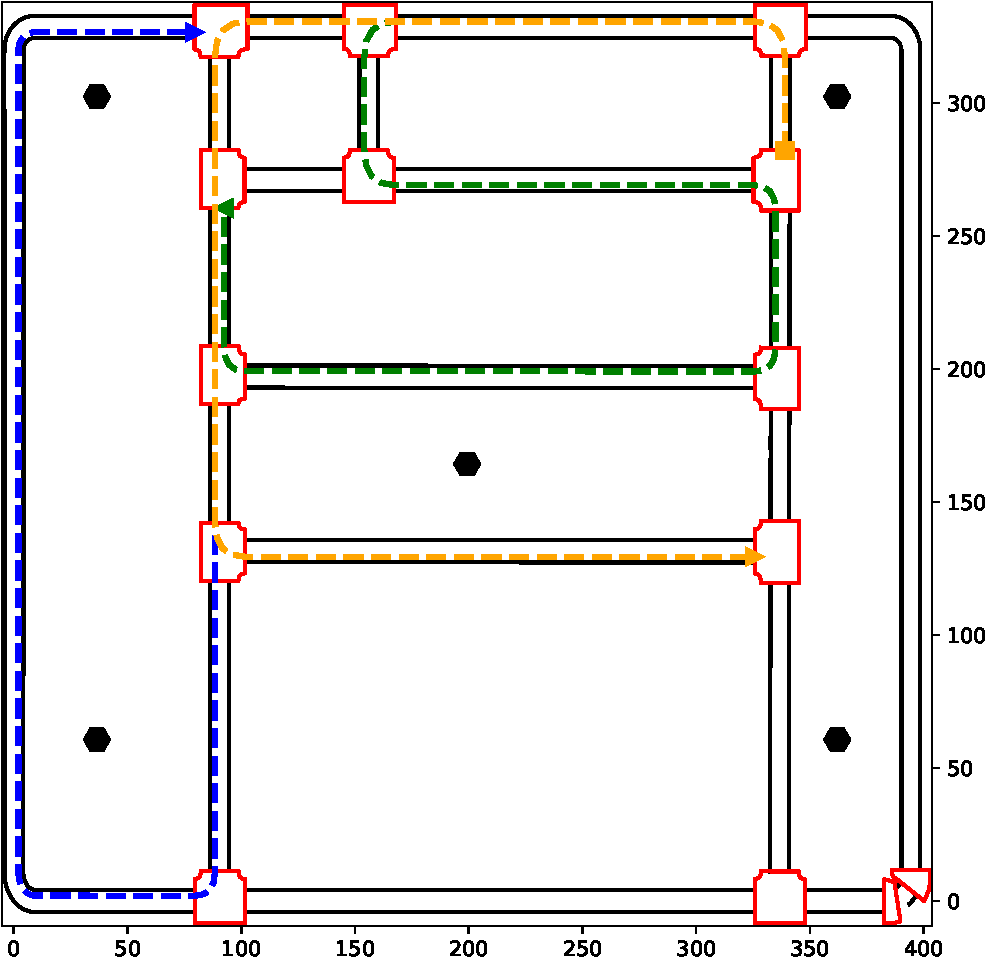
\includegraphics[width=1.0\textwidth]{chapter2/fig_traffic_map.pdf}
    \caption{The illustration of {\IAV} paths and BS locations on the road map.}
    \label{fig:traffic_map}
\end{figure*}

As for the performance benchmarks, we compare the proposed {\fwName} optimizer with the following ones.
\begin{itemize}
    \item \textbf{Equal-time Policy}:The one where all the {\IAVs} choose the maximum transmission power $P_{\max}$ and equal time allocation.
    % \item \textbf{Time-efficient Policy}: The one chooses the best channel conditioned one to transmit at each time slot, i.e., $\gamma_{m',t}=1$, $p_{m',t} = P_{\max}$, where $m' = \arg\min_{m} l_{m,t}$, $\forall t$.
    \item \textbf{Equal-rate Policy}: {The one chooses the best channel conditioned one to transmit at each time slot, i.e., $\gamma_{m',t}=1$, $p_{m',t} = P_{\max}$, where $m' = \arg\min_{m} l_{m,t}$, $\forall t$.}
    \item \textbf{One-shot Policy}: The one solves problem \textbf{P2$(k)$} once at the very start and then adopts the same policy for all the remaining time slots.
    % \item \textbf{Super-slot Only}: The one solves problem \textbf{P2$(k)$} at the start of every super slot, and adopts the same policy intermediately.
    \item \textbf{Exhaustive Policy}: The one optimizes problem \textbf{P2$(k)$} exhaustively at each time slot, i.e., $N=1$ in the {\fwName} optimizer;
    \item \textbf{Proposed Policy}: The one solves global and local optimization problems in the proposed {\fwName} optimizer alternatively with $N=5$.
\end{itemize}

\subsection{Performance Analysis}
\label{subsec:chapter2-performance}
First of all, we demonstrate how the transition of the {\IAV} locations is extracted as Markov transition chain in \figurename~\ref{fig:analyze_markov_chain}.
As shown in \figurename~\ref{fig:analyze_markov_chain}, the delta of transition changes periodically along the time slots, and the transition chain is stationary within around every 100 seconds.
\begin{figure*}
    \centering
    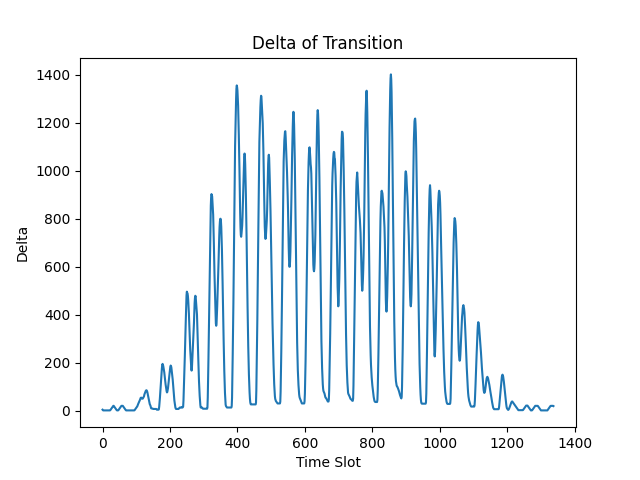
\includegraphics[width=1.0\textwidth]{chapter2/analyze_markov_chain.png}
    \caption{The stationary Markov transition chain of the {\IAV} locations.}
    \label{fig:analyze_markov_chain}
\end{figure*}

The total weighted cost of the proposed {\fwName} optimizer and the benchmarks are illustrated in the bar graph in \figurename~\ref{fig:analyze_total_cost}.
\begin{figure*}
    \centering
    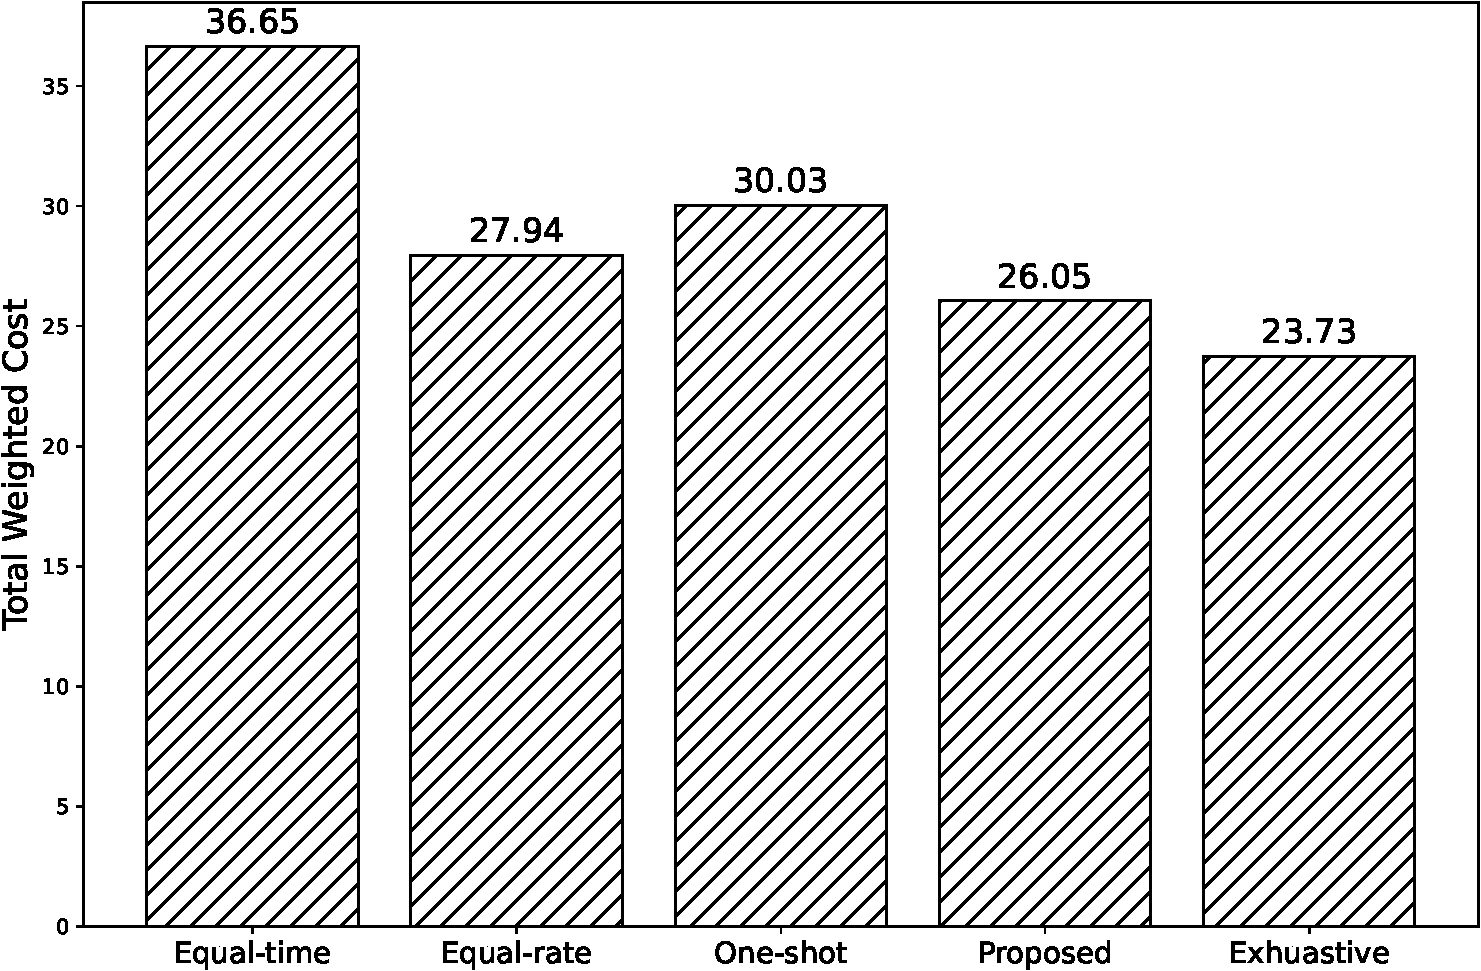
\includegraphics[width=1.0\textwidth]{chapter2/analyze_cost_bar.pdf}
    \caption{The total weighted cost of the proposed {\fwName} optimizer and the benchmarks.}
    \label{fig:analyze_total_cost}
\end{figure*}

\revise{
    It can be observed that the average overall cost of the {\fwName} optimizer is significantly better than the equal-time policy and the best-channel policy. The performance gain of the proposed {\fwName} optimizer over the decoupled policy is due to periodic optimization of problem \textbf{P2}.
}%
To further demonstrate the performance gap between the proposed {\fwName} optimizer and the benchmarks, we also plot the accumulated weighted cost versus time slots in \figurename~\ref{fig:analyze_accumulated_cost}.
\begin{figure*}
    \centering
    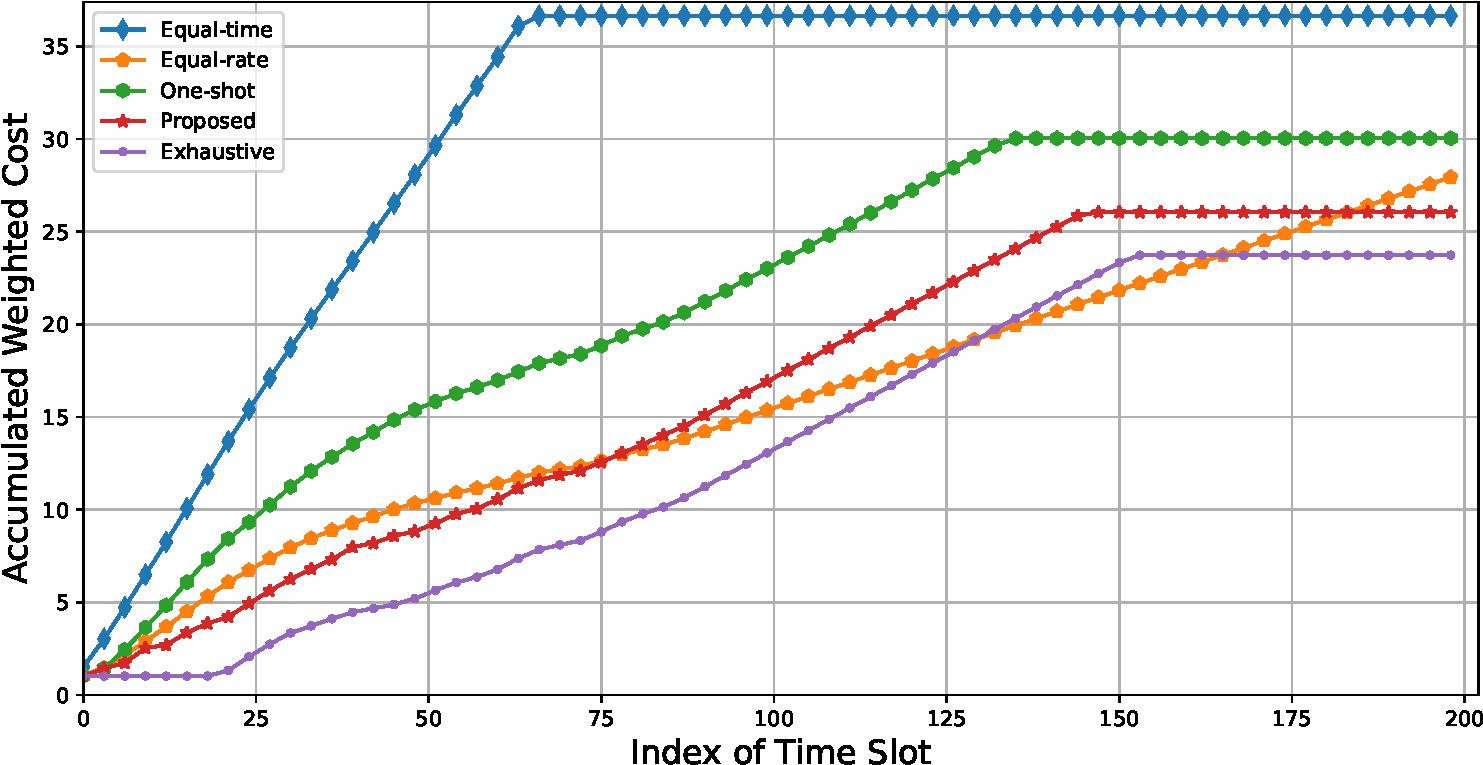
\includegraphics[width=1.0\textwidth]{chapter2/analyze_accumulated_cost.pdf}
    \caption{The accumulated weighted cost versus time slots.}
    \label{fig:analyze_accumulated_cost}
\end{figure*}

\subsection{Sensitivity Study}
\label{subsec:chapter2-sensitivity}
\noindent\textbf{Super slot Length $N$.}
The value function curve versus timeline w.r.t. various representative $N$ values.
\begin{figure*}
    \centering
    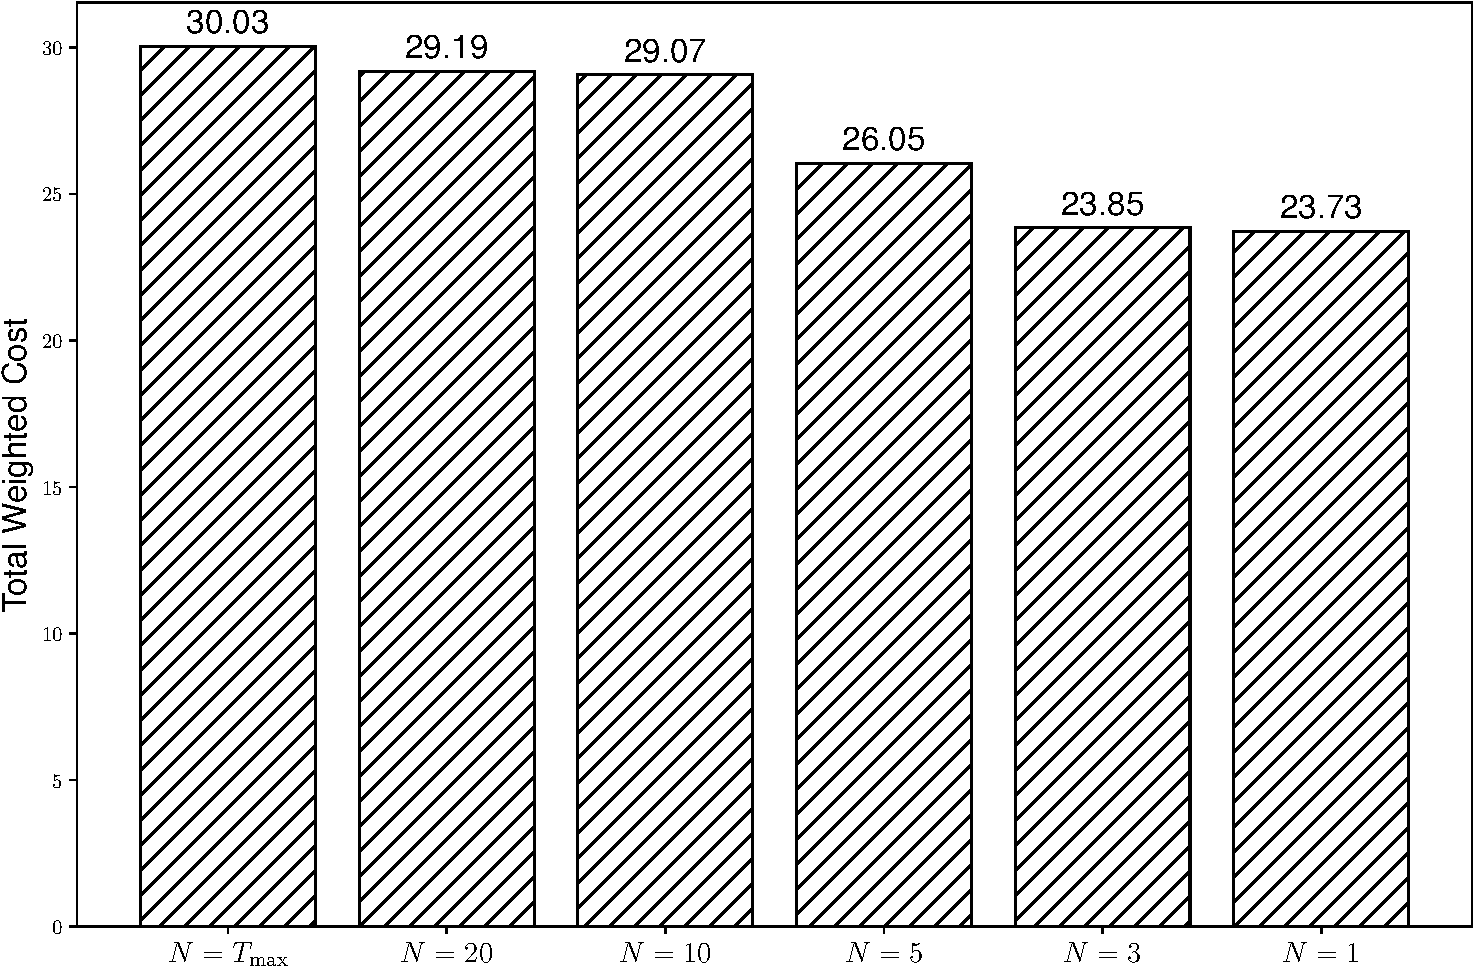
\includegraphics[width=1.0\textwidth]{chapter2/study_super_slot.pdf}
    \caption{The total weighted cost w.r.t different super slot length $N$.}
    \label{fig:study_super_slot}
\end{figure*}
The results show that smaller $N$ leads to better performance but higher computational complexity.


\noindent\textbf{Pareto Optimality}
The parameter $\omega$ tuning for balance of time-efficiency and energy-efficiency.
We sample different $\omega$ values and plot the Pareto curve.
\begin{figure*}
    \centering
    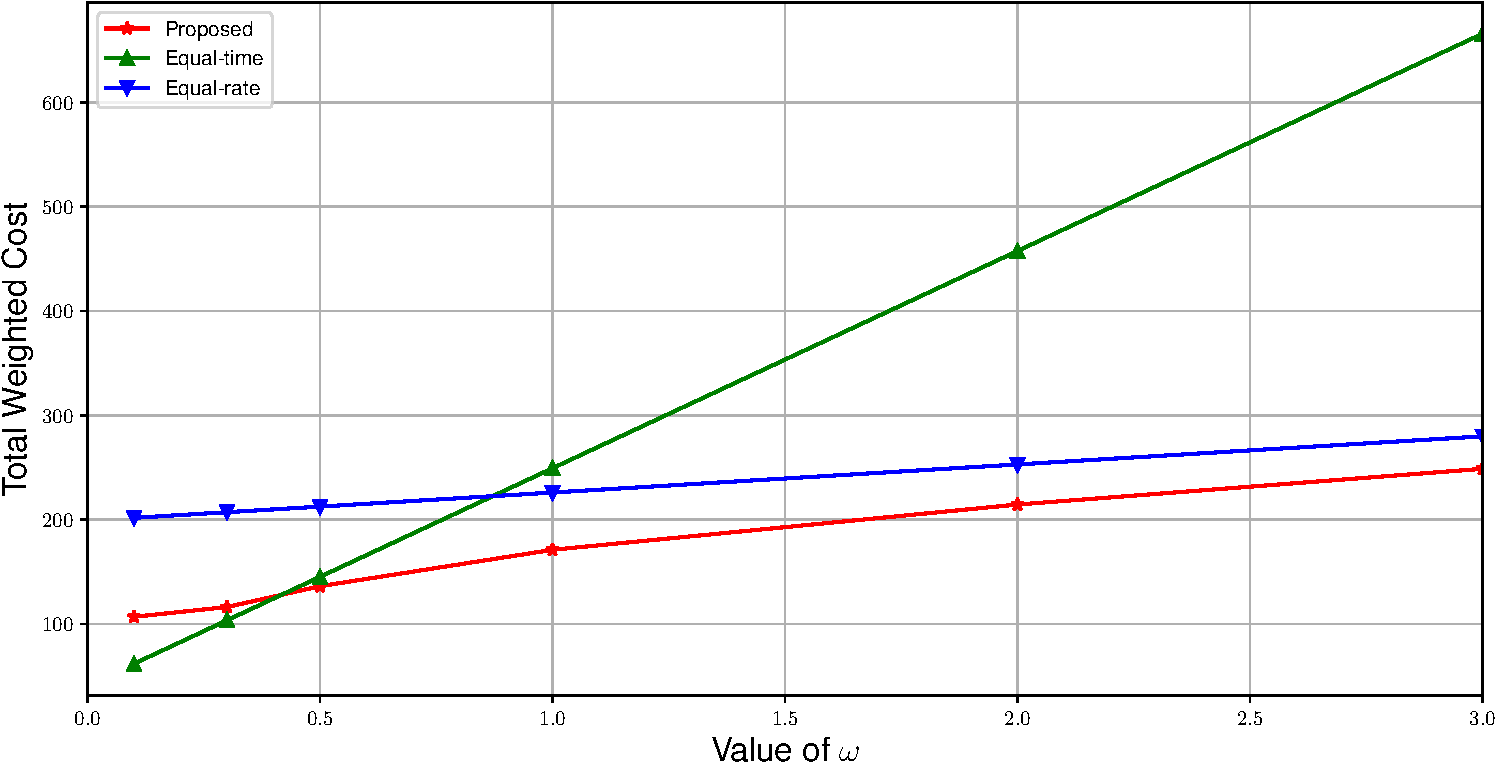
\includegraphics[width=1.0\textwidth]{chapter2/study_pareto_optimal.pdf}
    \caption{The total weighted cost under different weight $\omega$ and different algorithms.}
    \label{fig:study_pareto_optimal}
\end{figure*}
The results show that the proposed algorithm is Pareto optimal.

\noindent\textbf{Heterogeneity of Computation Capability.}
(1) all starts at same time, i.e., $T_{\text{comp},m}=0$, $\forall m\in\carSet$;
(2) only the driving-towards-BS ones starts earlier;
(3) only the driving-towards-BS ones starts later.
The results show that the proposed algorithm is robust to the heterogeneity of computation capability.


\section{Summary}
\label{sec:chapter2-conclusion}
We propose a data-driven framework called {\fwName} to study the communication scheduling problem for federated learning in vehicular networks.
The proposed {\fwName} framework is composed of two components: the high-fidelity trajectory dataset simulator and the {\fwName} optimizer.
In the {\fwName} trajectory simulator, we model the trajectory of each {\IAV} as a time-invariant Markov chain, and then formulate the communication scheduling problem as a finite-horizon MDP.
Since the optimal solution of the MDP suffers from the curse of dimensionality, we propose the {\fwName} optimizer to solve the problem in a low-complexity manner.
Specifically, every $N$ time slots are aggregated as \emph{super slot}.

The {\fwName} optimizer first determines the optimal time allocation policies for the remaining time slots at the beginning of each super slot.
Then, the {\fwName} optimizer determines the optimal power policies for each time slot for each {\IAV} independently.
The simulation results show that the proposed {\fwName} optimizer can achieve near-optimal performance with low complexity, and flexible trade-off between the performance and the computational complexity.
Furthermore, the hand-over among multiple base stations and the scheduling of multiple training epochs are not taken into consideration.
